\documentclass[12pt]{article}

\usepackage{amsmath,amsthm}
\usepackage{newtxtext,newtxmath}
\usepackage{booktabs}
\usepackage{graphicx}
\usepackage[letterpaper,margin=0.9in]{geometry}
\usepackage{xcolor}
\usepackage{float}
\usepackage{caption}
\usepackage{scicite}
\usepackage{url}
\frenchspacing

\renewcommand\refname{References and Notes}
\renewcommand{\thefigure}{S\arabic{figure}}
\renewcommand{\thetable}{S\arabic{table}}
\renewcommand{\thepage}{S\arabic{page}}

\makeatletter
\renewcommand{\fnum@figure}{\textbf{Figure \thefigure}}
\renewcommand{\fnum@table}{\textbf{Table \thetable}}
\makeatother

\begin{document}
\sloppy
\emergencystretch=1.5em

% Lock exact citation numbering 1..49 to match science_main.pdf identically:
\nocite{fitch1971toward,felsenstein1981evolutionary,saitou1987neighbor,price2010fasttree,kozlov2019raxml,minh2020iqtree,rissanen1978modeling,rissanen1983universal,felsenstein1985confidence,kosakovskypond2006gard,rokas2006animal,shen2017contentious,abadi2019model,felsenstein1978cases,yang1994maximum,le2008improved,doolittle1999phylogenetic,worobey1999widespread,liu2010convergent,parker2013genome,zou2015no,turakhia2022pandemic,malovichko2026toga2,jain1999horizontal,parks2020gtdb,dewitt2026gcreplay,morita2020clonal,methods,zhang2025aster,jarvis2014whole,prum2015comprehensive,wickett2014phylotranscriptomic,misof2014phylogenomics,chen2015identifying,borowiec2015extracting,whelan2017ctenophore,song2012resolving,shultz2019widespread,thomas2015molecular,christin2012adaptive,lytras2022exploring,wyres2020population,castelle2018major,mcdonald2012greengenes,tas2016visualizing,dewitt2018gctree,sollier2023compass,salehi2023sitka,bushwhacker_code}

\begin{center}
\section*{Supplementary Materials for\\ \bfseries \boldmath Evolutionary history from genomes to single cells by lossless compression}

Sergei~L.~Kosakovsky~Pond$^\ast$, Darren~P.~Martin, Stephanie~J.~K.~Pond, Steven~Weaver, Danielle~Callan, and~Anton~Nekrutenko\\[0.4em]
\small $^\ast$Corresponding author. Email: spond@temple.edu
\end{center}

\bigskip
\hrule
\medskip
\subsubsection*{This PDF file includes:}
Materials and Methods\\
Supplementary Text (Sections S1 to S6)\\
Figs.~S1 to S7\\
Tables~S1 to S11\\
References and Notes (References \textit{1} to \textit{49} match the main text; References \textit{50} to \textit{91} are cited only in the Supplementary Materials)
\medskip
\hrule
\bigskip

% ============================================================================
\section*{Materials and Methods}
% ============================================================================

\subsection*{Two-Part Minimum Description Length Objective and Star-Tree Null Baseline}

In probabilistic phylogenetics, a substitution model and tree $T$ assign a joint likelihood $P(A \mid T)$ to a discrete character matrix or multiple sequence alignment $A \in \Sigma^{N \times L}$ over $N$ taxa (or single cells) and $L$ columns on alphabet $\Sigma$ \cite{felsenstein1981evolutionary}. By Shannon's source coding theorem, $-\ln P(A \mid T)$ equals the exact code length in nats ($1\text{ nat} = 1/\ln 2 \approx 1.4427\text{ bits}$) required to transmit $A$ conditional on $T$. Standard model-selection criteria such as AIC and BIC \cite{akaike1974new,schwarz1978estimating,posada2004model,kalyaanamoorthy2017modelfinder} penalize the $1$ to $10$ continuous parameters of a rate matrix $Q$ while leaving the $(N-3)$ discrete bipartition choices of $T$ unpriced \cite{box1976science,susko2020use}. Under Rissanen's two-part Minimum Description Length (MDL) principle \cite{rissanen1978modeling,rissanen1983universal}, both the evolutionary graph $\mathcal{G} = (V, E_{\text{tree}}, E_{\text{shunt}})$ and the data encoded along it share one unit: $\mathcal{L}_{\text{MDL}}(A, \mathcal{G}) = \mathcal{L}(\mathcal{G}) + \mathcal{L}(A \mid \mathcal{G})$.

To establish an assumption-free null baseline, we price $A$ on an unresolved star phylogeny $T_{\text{star}}$ containing zero internal splits. Sending raw ungapped entries independently costs $N L_{\text{eff}}\ln|\Sigma|$ nats, whereas sending one ancestral root vector $X_r \in \Sigma^L$ costs $L\ln|\Sigma|$ nats plus, on each terminal branch $i \in \{1,\dots,N\}$, only the $m_i$ positions where lineage $i$ differs across its $L_{\text{eff},i}$ observed columns:
\begin{equation}
    \mathcal{L}_{\text{branch}}(m_i, L_{\text{eff}, i}) \;=\; \mathcal{L}_{\mathbb{N}}(m_i) + \ln\binom{L_{\text{eff}, i}}{m_i} + \sum_{k=1}^{m_i} \ell_{\text{subst}}(a_{i,k} \to b_{i,k}),
    \label{eq:branch_code}
\end{equation}
where $\mathcal{L}_{\mathbb{N}}(0) = \ln 2$ and, for $m_i \ge 1$,
\[
    \mathcal{L}_{\mathbb{N}}(m_i) \;=\; -\ln\!\left[\frac{\ln 2}{2}\!\left(\frac{1}{\ln(m_i+1)} - \frac{1}{\ln(m_i+2)}\right)\right]
\]
is the Kraft-tight Elias--Rissanen universal integer code \cite{rissanen1983universal} satisfying $\sum_{m=0}^{\infty} e^{-\mathcal{L}_{\mathbb{N}}(m)} = 1$ identically without any separate active-branch indicator bit; $\ln\binom{L_{\text{eff}, i}}{m_i}$ indexes which unordered subset of $m_i$ columns mutated (vanishing at $m_i = 0$); and $\ell_{\text{subst}}(a \to b) = -\ln P(b \mid a)$ is the Kraft-normalized substitution surprise ($\sum_{b \neq a} e^{-\ell_{\text{subst}}(a \to b)} = 1$). Summing Eq.~\eqref{eq:branch_code} over $X_r$ and all leaves yields $\mathcal{L}_{\text{MDL}}(A, T_{\text{star}})$ and the dimensionless Phylogenetic Compression Ratio:
\begin{equation}
    \rho(A) \;=\; 1 - \frac{\mathcal{L}_{\text{MDL}}(A, \mathcal{G}^*)}{\mathcal{L}_{\text{MDL}}(A, T_{\text{star}})}.
    \label{eq:comp_ratio}
\end{equation}

\subsection*{Exact Bipartition Cost, Rate Weighting, and the Natural Polytomy Law}

Splitting a multifurcating hub $w$ of degree $d = k_u + k_v \ge 4$ by inserting branch $e = (u,v)$ partitions its $d$ incident lineages into $2 \le k_u \le k_v$ children. Indexing the unordered split size $\{k_u, k_v\}$ among $\max(1, \lfloor d/2\rfloor - 1)$ non-trivial choices and selecting the $k_u$-subset (halved by symmetry when $k_u = k_v$) incurs the exact topological address cost:
\begin{equation}
    \mathcal{L}_{\text{topo}}(k_u, k_v) \;=\; \ln\,\max\!\left(1,\; \left\lfloor\frac{k_u + k_v}{2}\right\rfloor - 1\right) \;+\; \ln\binom{k_u + k_v}{k_u} \;-\; \mathbb{I}(k_u = k_v)\ln 2 \quad \text{nats}.
    \label{eq:topo_cost}
\end{equation}
For a quartet ($k_u = k_v = 2$), $\mathcal{L}_{\text{topo}}(2,2) = \ln 3 \approx 1.099\text{ nats}$; within a degree-$d$ burst hub, $\mathcal{L}_{\text{topo}}(2, d-2) \approx 3\ln d - 2\ln 2$ automatically corrects for searching across all $\binom{d}{2}$ pairs (unlike purely local edge tests \cite{anisimova2011survey,hoang2018ufboot2}). Shifting one shared derived edit off an adjacent branch $c$ carrying $m_c$ mutations reduces its positional subset cost by
\begin{equation}
    w_c \;=\; \ln\binom{L_{\text{eff}}}{m_c + 1} - \ln\binom{L_{\text{eff}}}{m_c} \;=\; \ln\!\left(\frac{L_{\text{eff}} - m_c}{m_c + 1}\right) \;\approx\; -\ln\!\left(\frac{p_c}{1 - p_c}\right) \quad \text{nats},
    \label{eq:marginal_weight}
\end{equation}
recovering Felsenstein's exact maximum-likelihood log-odds branch weight \cite{felsenstein1981evolutionary}. Writing $\Delta\mathcal{L}_{\text{children}}(m)$ for the child-branch code savings when $m$ shared edits are factored onto $e$, split $e$ is retained if and only if its net MDL compression gain is positive:
\begin{equation}
    G_{\text{MDL}}(e) \;\equiv\; -\Delta\mathcal{L}_{\text{MDL}}(e) \;=\; \max_{1 \le m \le K} \Big[ \Delta\mathcal{L}_{\text{children}}(m) - \mathcal{L}_{\text{branch}}(m, L_{\text{eff}}) \Big] - \mathcal{L}_{\text{topo}}(k_u, k_v) \;>\; 0,
    \label{eq:mdl_gain}
\end{equation}
which maps directly onto a conditional local posterior branch probability $P_{\text{local}}(e \mid T_{-e}, A) = \big(1 + \exp(-G_{\text{MDL}}(e))\big)^{-1}$ comparing the locally optimal split state against collapsing $e$ on the fixed surrounding topology $T_{-e}$ without bootstrap resampling \cite{felsenstein1985confidence}.

\subsection*{Four-Stage Hybrid Compression and Graph Induction Architecture}

Finding the global MDL minimum across all $(2N-5)!!$ leaf-labeled topologies is NP-hard, so Bushwhacker executes a deterministic four-stage search combining sub-quadratic distance/Voronoi seeding, vectorized continuous-time (\texttt{GTR+CAT8}/\texttt{LG08+CAT8}) or discrete/ordered (\texttt{--discrete}/\texttt{--ordered}) local optimization, post-hoc MDL contraction, and lateral shunt peeling:
\begin{enumerate}
    \item \textbf{Bit-Parallel Encoding and Empirical Exchange Costs:} Nucleotide states and IUPAC ambiguities pack into four 64-bit integer bitplanes (\texttt{[u64; 4]}) per 64 alignment columns; variable-site patterns deduplicate deterministically by run-length encoding. Empirical transition ($\hat{p}_{\text{ti}}$) and transversion ($\hat{p}_{\text{tv}} = 1 - \hat{p}_{\text{ti}}$) costs ($\ell_{\text{ti}} = -\ln\hat{p}_{\text{ti}}$, $\ell_{\text{tv}} = -\ln(\hat{p}_{\text{tv}}/2)$) and empirical GTR/LG08 Markov parameters parameterize the discrete ledger and continuous-time likelihood sweeps.
    \item \textbf{Stage 1 --- Sub-Quadratic Starting Scaffold ($T_0$):} On a stratified pilot subsample ($K_{\text{sub}} \le 128$), sitewise Fitch edit counts $s_k$ \cite{fitch1971toward} under Poisson saturation $m_k = -k_{\text{sat}}\ln(1 - \min(0.92, s_k / k_{\text{sat}}))$ estimate the Gamma rate-dispersion shape $\hat{\alpha} \in [0.15, 50.0]$ and Jin--Nei ($\text{K80}+\Gamma(\hat{\alpha})$) distances \cite{jin1990limitations}:
    \begin{equation}
        \begin{aligned}
            \hat{\alpha} &\;=\; \frac{\bar{m}^2}{\max\!\big(10^{-6},\; \text{Var}(m) - \bar{m}\big)}, \\
            M_{ij} &\;=\; L_{ij} \cdot \frac{\hat{\alpha}}{2}\!\left[ (1 - 2P_{ij} - Q_{ij})^{-1/\hat{\alpha}} + \frac{1}{2}(1 - 2Q_{ij})^{-1/\hat{\alpha}} - \frac{3}{2} \right].
        \end{aligned}
        \label{eq:jin_nei}
    \end{equation}
    For $N \le 4{,}096$, BioNJ builds the binary starting scaffold $T_0$ from the distance matrix; for $N > 4{,}096$, Voronoi landmark divide-and-conquer partitions taxa and builds an $\mathcal{O}(N\log N \cdot L/64)$ skeleton \cite{guindon2010new}.
    \item \textbf{Stage 2 --- Continuous-Time Rate-Category and Discrete Topology Refinement:} On all default nucleotide ($N \ge 4$) and protein/translated ($N \ge 3$) alignments, Bushwhacker assigns each variable column $s$ unconditionally by nearest log-rate to one of eight unit-mean $\Gamma(1,1)$ octile rate categories ($r_1, \dots, r_8$, $\frac{1}{8}\sum_{k=1}^8 r_k = 1$) and runs a fixed deterministic schedule (\texttt{NNI + LeafMLE + SPR2 + NNI}) over 64-pattern SoA cache tiles (\texttt{GTR+CAT8} or \texttt{LG08+CAT8}): local \texttt{NNI} swaps accept Fisher-curvature-penalized log-likelihood gains $\Delta\text{MDL} > 0.01\text{ nats}$, while 15-topology \texttt{SPR2} quintet moves accept log-likelihood gains $\Delta\ln P > 0.05\text{ nats}$ to prevent numerical oscillation. Under \texttt{--discrete} and \texttt{--ordered}, Stage~2 instead optimizes the exact discrete/ordered MDL objective directly via postorder/preorder Sankoff--Fitch/interval sweeps.
    \item \textbf{Stage 3 --- Deterministic Polytomy Contraction and Discrete Hub Expansion:} Internal branches contract sequentially from most negative gain upward when $G_{\text{MDL}}(e) \le 0$. On default continuous-time \texttt{GTR+CAT8}/\texttt{LG08+CAT8} paths, branch contraction tests $\Delta\ln P(e) - \big[\frac{1}{2}\ln\max(1, m_{\text{var}}/2\pi) + \frac{1}{2}\ln\max(1, N-3) + \mathcal{L}_{\text{topo}}(k_u, k_v)\big] \le 0$ and emits the contracted graph (alongside the pre-contraction binary refinement via \texttt{-b}) without running multi-taxon clique expansion; on \texttt{--discrete} and \texttt{--ordered} inputs, degree-$d$ hubs additionally propose multi-taxon splits ($2 \le k_u \le d-2$) retained whenever $G_{\text{MDL}}(e) > 0$.
    \item \textbf{Stage 4 --- Dual-Mode Lateral Shunt Peeling:} Residual non-sister parallel substitutions $S_{u,v} = \{s_1, \dots, s_m\}$ (pooled across up to three consecutive ancestral coding branches while excluding ancestral symplesiomorphies) are tested as lateral links $h = (u \to v)$ priced by endpoint address $2\ln|V|$ plus the shorter of contiguous-tract (\texttt{INTERVAL}) or scattered-site (\texttt{SPARSE}) mask codes:
    \begin{equation}
        \begin{aligned}
            \mathcal{L}_{\text{mask}}^{\text{INTERVAL}}([a,b]) &\;=\; \ln 2 + 2\ln L + \mathcal{L}_{\text{branch}}(d_{[a,b]}, b - a + 1), \\
            \mathcal{L}_{\text{mask}}^{\text{SPARSE}}(S_{u,v}) &\;=\; \ln 2 + \ln\binom{M_{\text{pool}}}{m} + \mathcal{L}_{\mathbb{N}}(m - m_{\min}),
        \end{aligned}
        \label{eq:shunt_masks}
    \end{equation}
    where $d_{[a,b]}$ counts discordant positions in $[a,b]$, $M_{\text{pool}} \le L$ is the size of the address space from which the $m$ parallel sites are drawn---the number of variable alignment columns for non-coding nucleotide, protein, and somatic alignments, and the number of amino-acid-variable codons (positions with $\ge 2$ distinct residues; $302$ of $745$ codons in mammalian \textit{Prestin}) for coding/translated alignments, matching the codon-level unit at which parallel coding substitutions are enumerated---and $m_{\min} = 2$ (nucleotide) or $4$ (protein) is the structural minimum site threshold with Elias-delta / universal integer prefix code $\mathcal{L}_{\mathbb{N}}$ ensuring Kraft-exact self-delimiting completeness across shunt cardinalities (empirically producing $0/50$ new shunts on both 20-state AA and nucleotide zero-shunt TOGA2 controls). To guard against tearing genuine vertical tree splits on noisy tracts, Stage~4 masks recipient nucleotides only for contiguous \texttt{INTERVAL} transfers whose MDL gain exceeds $15\text{ nats}$ ($e^{-15} \approx 3\times 10^{-7}$ false-masking odds) before running Stage~3 re-verification.
\end{enumerate}

\subsection*{Multi-Alphabet Generalization and Continuous-Time Rate-Category Cache Tiling}

Bushwhacker extends Eqs.~\eqref{eq:branch_code}--\eqref{eq:shunt_masks} natively across discrete alphabets:
\begin{itemize}
    \item \textbf{20-State Amino-Acid Alignments (\texttt{--protein} / \texttt{--translate}):} Twenty amino-acid bitplanes (\texttt{[u64; 20]} per 64 columns) and six Dayhoff--Miyata biochemical classes \cite{dayhoff1978model} yield empirical conservative probability $\hat{p}_{\text{cons}}$ (estimated from pairs with divergence $\le 0.35$) and normalized substitution costs:
    \begin{equation}
        \ell_{\text{subst}}^{\text{AA}}(a \to b) \;=\;
        \begin{cases}
            -\ln\!\big(\hat{p}_{\text{cons}} / k_{\text{same}}(a)\big), & \text{if } \text{class}(b) = \text{class}(a), \\[2pt]
            -\ln\!\big((1 - \hat{p}_{\text{cons}}) / k_{\text{diff}}(a)\big), & \text{if } \text{class}(b) \neq \text{class}(a).
        \end{cases}
        \label{eq:aa_subst}
    \end{equation}
    \item \textbf{Discrete Single-Cell Somatic Matrices (\texttt{--discrete}, $2 \le K \le 32$):} Binary somatic SNV profiles ($0 = \text{WT}$, $1 = \text{mutant}$, $?/\texttt{-} = \text{allelic dropout}$) assign full wildcard bitmasks ($2^K - 1$) to missing entries, incurring zero dropout penalty while adjusting $L_{\text{eff}, i}$ per cell.
    \item \textbf{Ordered Zygosity and Copy-Number Profiles (\texttt{--ordered}, $3 \le K \le 16$):} Somatic zygosity states ($0 = \text{WT}$, $1 = \text{HET}$, $2 = \text{HOM/CN-LOH}$ \cite{morita2020clonal,sollier2023compass}) and DLP+ copy-number bins ($0, 1, \dots, 11+$ \cite{salehi2023sitka}) replace unordered Fitch intersections with exact linear-time $L_1$ interval propagation: parent interval $[l_1,r_1] \cap [l_2,r_2]$ if overlapping, or $[\min(r_1,r_2), \max(l_1,l_2)]$ otherwise, paired with geometric step costs $\ell_{\text{step}}(\Delta s) = -\ln\big((1-\hat{q})\hat{q}^{|\Delta s|-1}/Z_a\big)$. On $500\text{-kb}$ bin matrices ($4,375$ bins), Bushwhacker supports raw bin compression with root run-length chromosomal coding and lossless breakpoint-segment aggregation ($365\text{--}448$ multiplicity-weighted segments).
    \item \textbf{Continuous-Time Hard-CAT Rate Models with 64-Site Cache Tiling (\texttt{GTR+CAT8} / \texttt{LG08+CAT8}):} Running unconditionally on nucleotide ($N \ge 4$) and protein/translated ($N \ge 3$) alignments \cite{tavare1986some,yang1994maximum,le2008improved}, continuous-time reversible Markov models assign each variable column $s$ unconditionally by nearest log-rate to one of eight fixed categories ($r_1, \dots, r_8$; analytical octile means of $\Gamma(1,1)$ satisfying $\frac{1}{8}\sum_{k=1}^8 r_k = 1$):
    \begin{equation}
        \begin{aligned}
            G_{\text{CT-MDL}}(e) &\;=\; \Delta\ln P(e \mid T, r_{k^*(\cdot)}\hat{\mathbf{t}}, Q_M) \\
            &\qquad \;-\; \left[ \frac{1}{2}\ln\max\!\left(1,\frac{m_{\text{var}}}{2\pi}\right) + \frac{1}{2}\ln\max(1, N-3) + \mathcal{L}_{\text{topo}}(k_u, k_v) \right],
        \end{aligned}
        \label{eq:ct_mdl}
    \end{equation}
    evaluated over cached transition matrices $P(t) = U\operatorname{diag}(e^{\lambda r_k t})U^{-1}$ on a 15-point log-spaced branch-length grid with parabolic curvature refinement ($\frac{1}{2}\ln(1 + \mathcal{I}(e)/2\pi)$ during NNI scoring), contracting silent stems smoothly when $G_{\text{CT-MDL}}(e) \le 0$. Partitioning unique site patterns into $B = 64$-pattern L1/L2 cache tiles bounds resident likelihood memory at $\mathcal{O}(N \cdot B \cdot C \cdot |\Sigma|)$ ($1.98\text{--}2.71\text{ GB}$ across mammalian and prokaryotic marker corpora, and $4.07\text{ GB}$ at $32,768$ taxa vs.\ $26.37\text{--}79.15\text{ GB}$ for standard likelihood engines; Table~\ref{tab:tol_sota}). Controlled four-mode ablations (\texttt{--no-mult-pen} omitting $\frac{1}{2}\ln\max(1, N-3)$ and \texttt{--empirical-alpha} estimating discrete $\alpha$ in place of $\Gamma(1,1)$; Section~S2 and Table~\ref{tab:tol_sota}) verify that both architectural choices remain empirically necessary and non-fragile. In JSON output, \texttt{tree\_MDL\_nats} records the unified discrete branch-edit summary code (Eq.~\eqref{eq:branch_code} evaluated at continuous-time-informed branch loads $\max(\hat{t}_e \bar{r}_{\text{emp}} L_{\text{eff}}, m_e)$), whereas topological contraction on nucleotide and protein alignments evaluates the continuous-time criterion of Eq.~\eqref{eq:ct_mdl} directly.
\end{itemize}

\subsection*{Lossless \texttt{.bwz} Causal Phylogenetic Arithmetic Codec}

Invoked via \texttt{bushwhacker -c} and \texttt{-d}, the \texttt{.bwz} archiver encodes taxon identifiers, the Newick graph, the root sequence (with Markov run-length coding for indel and dropout runs), and causal preorder branch deltas using 32-bit arithmetic coding \cite{witten1987arithmetic} conditioned on empirical site-rate and codon-phase priors, guaranteeing bit-exact FASTA reconstruction (\texttt{SHA-256} verified across Table~\ref{tab:compression_codec}).

\subsection*{Computational Environment, Baseline Software, and Multiple-Testing Governance}

\begin{itemize}
    \item \textbf{Implementation and Determinism:} Bushwhacker is written in native Rust (\texttt{rustc 1.94.1}) with zero external C/C++ dependencies and compiles to both a multi-threaded CLI binary (\texttt{-T/--threads}, bit-exact identical across $1\text{--}64$ threads with fixed seed \texttt{20261112} and zero random tie-breaking) and client-side WebAssembly (\texttt{bushwhacker\_bg.wasm}). Open-source code, specimen files, reproducibility scripts, and browser UI reside at \url{https://github.com/veg/bushwhacker} and \url{https://veg.github.io/bushwhacker/}.
    \item \textbf{Compute Hardware:} All 32-core Tree-of-Life supermatrices, Greengenes 16S scaling runs, pandemic viral alignments, and coalescent cluster sweeps ran on an ARM64 Neoverse-N1 Linux server (64 cores, pinning 32 threads per method in head-to-head comparisons unless noted, with identical hardware wall-clock quotas and no timeouts bypassed). Single-cell cancer phylogenomics, specimen reconstructions, and \texttt{.bwz} archive verifications ran on an Apple M5 Max workstation (18-core CPU, 36~GB unified memory, macOS).
    \item \textbf{External Baseline Software:} Baselines were executed with \texttt{IQ-TREE multicore v2.4.0} (\texttt{-m MFP}, \texttt{-m GTR+I+G4}, \texttt{-m GTR+G4 --fast}, \texttt{-m LG+G4 --fast}, \texttt{--polytomy}, \texttt{--abayes}, \texttt{-alrt 1000}, \texttt{-B 1000}, and \texttt{AliSim}), \texttt{FastTree}/\texttt{FastTreeMP v2.1.11} (\texttt{-nt -gtr}, \texttt{-lg}), \texttt{ASTRAL-IV} (\texttt{ASTER} \texttt{astral4} \texttt{-t 8}), \texttt{GCtree}, \texttt{COMPASS} \cite{sollier2023compass,jahn2016tree}, \texttt{HyPhy GARD}, \texttt{INDELible}, \texttt{gzip -9}, \texttt{bzip2 v1.0.8 -9}, and \texttt{xz}/\texttt{lzma} (\texttt{XZ Utils v5.8.1}, \texttt{-6}/\texttt{-9}), scored by exact bipartition Robinson--Foulds matching \cite{robinson1981comparison}.
    \item \textbf{Zero-Leakage, Multiple-Testing, and Ethics Governance:} Across every immune and cancer single-cell benchmark, cell multiplicities, DMS affinity scores, clinical timepoints, anatomic compartments, and passage numbers were stripped strictly prior to inference and linked solely post hoc. To control the false discovery rate (FDR) across all $31$ two-sided biological hypothesis tests audited across main text and supplement (including ecological guild, archaeal \texttt{ar122}, and negative-control screens), raw $p$-values were adjusted jointly using Benjamini--Hochberg (BH) step-up control ($\alpha_{\text{FDR}} = 0.05$): $24/31$ tests remain significant at $q < 0.05$, whereas all seven null/negative-control comparisons remain non-significant ($q_{\text{BH}} \ge 0.194$: non-multicopy ant-eating screen $p = 0.157, q = 0.194$; unadjusted marine/aquatic $p = 0.164, q = 0.196$; \texttt{ar122} Complexity Hypothesis $p = 0.213, q = 0.221$; subterranean blind $p = 0.214, q = 0.221$; pooled binary BCR hub-vs-nonhub DMS affinity $p = 0.203, q = 0.221$; Morita AML direct cell count vs.\ $k_{\text{out}}$ $p = 0.197, q = 0.221$; and DLP+ \texttt{SA535} passage aneuploidy $p = 0.475, q = 0.475$). This retrospective \textit{in silico} study analyzed only public de-identified datasets with zero wet-lab manipulation, human identifiers, or biosecurity concerns.
\end{itemize}

\subsection*{Data Provenance and Empirical Archive Identifiers}

\begin{enumerate}
    \item \textbf{Model-Selection Benchmark Archive ($7,200$ empirical + $27,500$ simulated alignments):} OSF repository \url{https://doi.org/10.17605/OSF.IO/T3PF2} \cite{abadi2019model,gerth2019cannot}, spanning PlantDB, Selectome, TreeBASE, and Pandora empirical loci alongside \texttt{INDELible} ground-truth suites \texttt{sim\_bic} ($n = 5,901$), \texttt{c0} ($n = 7,199$), \texttt{c1} ($n = 7,200$), and \texttt{c2} ($n = 7,200$).
    \item \textbf{Eukaryotic Phylogenomic Radiations ($19$ datasets, $45,205$ loci; $83,180$ multi-seed searches):} Figshare project \texttt{22040} (\url{https://figshare.com/projects/Evaluating_fast_maximum_likelihood-based_phylogenetic_programs_using_empirical_phylogenomic_data_sets/22040} \cite{shen2017contentious,zhou2018evaluating}), including mammalian \texttt{CHST13} ($22$ species, $1,176\text{ bp}$ from \texttt{TarvD7}), plus the whole-genome avian radiation (\texttt{Avian\_Shultz2019}; Dryad \url{https://doi.org/10.5061/dryad.4b8gt83} \cite{shultz2019widespread}; $50$ clean coding orthologs evaluated in \texttt{ASTRAL-IV} alongside $11$ radiation benchmarks \texttt{ChenA4}, \texttt{MisoA2}, \texttt{ShenA9}, \texttt{BoroA6}, \texttt{WickA3}/\texttt{WickD3a}, \texttt{NagyA1}, \texttt{SongD1}, \texttt{XiD4}, \texttt{PrumD6}, \texttt{WhelA7} totaling $12,008$ runs / $11,164$ distinct loci).
    \item \textbf{Mammalian \textit{Prestin} (\texttt{SLC26A5}) and TOGA2 882-Mammal Atlas:} Complete $116$-mammal \textit{Prestin} coding alignment ($2,235\text{ bp}$; \texttt{docs/examples/prestin.fasta} \cite{liu2010convergent,li2010hearing}), and the Senckenberg TOGA2 \texttt{hg38 v1} archive (\url{https://genome.senckenberg.de/download/TOGA2/MultiCodonAlignments/reference_human_hg38/v1/} \cite{kirilenko2023integrating,malovichko2026toga2}; $882$ assemblies across $20$ orders and $116$ families: $19,952$ coding alignments, $19,953$ translated proteins, $5,058$ de novo \texttt{WALRUS} codon MSAs with $1,487$ completed protein-shunt cross-checks, and the $253$-locus concatenated mammalian supermatrix).
    \item \textbf{Botanical and Poaceae $\text{C}_4$ Corpus ($2,002$ alignments):} Land-plant \texttt{WickD3a}/\texttt{WickD3b} ($1,688$ alignments \cite{wickett2014phylotranscriptomic}), seed-plant \texttt{XiD4} ($310$ genes \cite{xi2014coalescent}), GenBank plastid \texttt{rbcL\_483} ($483 \times 1,398\text{ bp}$), and Poaceae \texttt{ppc}, \texttt{pck}, and \texttt{rbcL} orthologs/paralogs including \textit{Alloteropsis semialata} $\text{C}_3$/$\text{C}_4$ copies retrieved from NCBI Entrez Nucleotide \cite{christin2007c4,christin2012adaptive,dunning2019pangenome}.
    \item \textbf{Prokaryotic Domains, Clinical \textit{K.\ pneumoniae}, and Greengenes 16S:} GTDB Release 95.0 (\url{https://data.gtdb.ecogenomic.org/releases/release95/95.0/} \cite{parks2018gtdb,parks2020gtdb}: \texttt{ar122} across $1,672$ archaea and $1,000$-species \texttt{bac120} across all $111$ phyla); clinical \textit{Klebsiella pneumoniae} genomes from NCBI BioProject \texttt{PRJNA246471} and RefSeq \cite{wyres2020population} ($16$-strain $214,038\text{-bp}$ core chromosome supermatrix, $222$ single-copy core loci across $10$ genomes, and matched $9$ clinical isolates---\texttt{CAV1016}, \texttt{CAV1042}, \texttt{CAV1193}, \texttt{CAV1344}, \texttt{CAV1392}, \texttt{CAV1453}, \texttt{CAV1596}, \texttt{HS11286\_ST11}, \texttt{NJST258\_2}---pairing the $214,038\text{-bp}$ chromosome against their $882\text{-bp}$ \textit{blaKPC} plasmid); \textit{S.\ pneumoniae} \texttt{PMEN1} ($11 \times 2.22\text{ Mb}$ \cite{croucher2011rapid}); and Greengenes \texttt{13\_5} 16S rRNA (\url{https://greengenes.secondgenome.com/} \cite{mcdonald2012greengenes}, $N = 256 \to 32,768 \times 1,348\text{ bp}$).
    \item \textbf{Pandemic Viral and \texttt{.bwz} Archives:} Open Nextstrain/GenBank SARS-CoV-2 (\url{https://data.nextstrain.org/files/ncov/open/}; $5,097$ and $10,062$ complete $29,903\text{-bp}$ genomes plus blinded Pango \texttt{X*} recombinants), global Dengue \texttt{DENV-1..4} ($1,426$, $2,632$, $855$, and $585$ coding genomes; $5,498$ total), LANL HIV-1 (\url{https://www.hiv.lanl.gov/}; \texttt{KAL153}, \texttt{CRF02\_AG}, \texttt{HIV1\_518} \cite{carr1998full,robertson2000hiv1}), bat sarbecoviruses (\texttt{Sarbeco\_83}, $83 \times 30,965\text{ bp}$ \cite{boni2020evolutionary,lytras2022exploring}), \texttt{InfluenzaA} HA ($349 \times 987\text{ bp}$), \texttt{Human\_mtDNA} ($78 \times 16,585\text{ bp}$), hominoid \texttt{MHC} ($379 \times 1,128\text{ bp}$ \cite{parham1996population}), and \textit{Heliconius} \texttt{optix} \cite{pardodiaz2012adaptive,dasmahapatra2012butterfly}.
    \item \textbf{Single-Cell Immune and Cancer Cohorts:} Mouse \texttt{CGG}-immunized germinal-center repertoires from \texttt{GCReplay} (\url{https://github.com/matsengrp/gcreplay} \cite{dewitt2026gcreplay}; $147$ GCs, $10,429$ paired \texttt{IGH+IGK} cells, $9,352$ unique $657\text{-bp}$ genotypes, plus $4,400$ scFv yeast-display $\Delta\log_{10} K_D$ scores) and \texttt{Clone\_3-8} ($66$ cells \cite{tas2016visualizing}); Mission Bio Tapestri myeloid scDNA runs from \texttt{COMPASS} (Zenodo \url{https://doi.org/10.5281/zenodo.10822292} \cite{sollier2023compass}; $168$ runs, $1,001,609$ cells) and the 123-patient AML cohort including specimen \texttt{AML-38-001} ($7,016$ cells, $11$ clones $\times 31$ loci, plus $7,016 \times 16$ raw single-cell Tapestri comparison against \texttt{COMPASS}; NCBI GEO \texttt{GSE146150} and Zenodo \url{https://zenodo.org/records/15096570} \cite{morita2020clonal}); and DLP+ scWGS copy-number matrices (\url{https://doi.org/10.24072/pcjournal.292} \cite{salehi2023sitka}; $4,950$ cells across \texttt{OV2295}, \texttt{SA501}, \texttt{SA609}, \texttt{SA535}).
    \item \textbf{Ground-Truth Synthetic Benchmarks ($36,920$ + $100$ GC histories):} \texttt{AliSim} 22-regime nucleotide suite ($220$ alignments \cite{lytrong2022alisim}), \texttt{Abadi/Gerth} nucleotide suite ($27,500$ alignments), \texttt{LG+G4} protein suite (\texttt{P1--P4}, $400$ alignments), deterministic Kingman Anomaly-Zone coalescent suite (\texttt{seed = 20261112}) ($8,000$ loci \cite{degnan2006discordance}) + $50$ Galton--Watson affinity-selected B-cell GCs + $50$ neutral ($\beta_{\text{bind}} = 0$) negative-control GCs (\texttt{MK\_RS5NF} 5-mer SHM \cite{dewitt2018gctree}), reticulate HGT/convergence suite (\texttt{N1--N4}, $400$ alignments), and single-cell SNV/CNA matrices (\texttt{C1--C4}, $400$ matrices).
\end{enumerate}

% ============================================================================
\section*{Supplementary Text}
% ============================================================================

\subsection*{Section S1: Why Two-Part Compression Resists Long-Branch Attraction and Enforces Polytomies}

Counting edits along branches superficially resembles unweighted maximum parsimony \cite{fitch1971toward}, which falls prey to long-branch attraction under rate heterogeneity \cite{felsenstein1978cases}. Eqs.~\eqref{eq:branch_code}--\eqref{eq:ct_mdl} prevent this artifact in three ways. First, Eq.~\eqref{eq:marginal_weight} weights every shifted mutation by $w_c = \ln\frac{L_{\text{eff}} - m_c}{m_c + 1}$: on our worked 4-taxon, 16-site quartet ($88.72\text{ nats}$ raw, $22.18\text{ nats}$ root, $61.02\text{ nats}$ star at $m_e = 0$ with $m_c = 2$ private leaf edits costing $\mathcal{L}_{\text{branch}}(2,16) = 9.71\text{ nats}$ each; Fig.~\ref{fig:supp_didactic} and Table~\ref{tab:synthetic_summary}), pooling a shared change from two quiet branches ($m_{\text{short}} = 1$, $w_{\text{short}} = 2.01\text{ nats}$) saves $4.03\text{ nats}$ versus $0.71\text{ nats}$ on two six-mutation branches ($w_{\text{long}} = 0.36\text{ nats}$)---a $5.6$-fold positional shield matching Felsenstein's likelihood weights \cite{felsenstein1981evolutionary}. Second, with $m_c = 2$ private edits per leaf ($\mathcal{L}_{\text{branch}}(1..4, 16) = 5.56, 9.71, 12.99, 15.72\text{ nats}$), one shared mutation saves $6.55\text{ nats}$ on the daughter branches yet costs $\mathcal{L}_{\text{branch}}(1,16) + \ln 3 = 6.66\text{ nats}$, contracting automatically ($G_{\text{MDL}} = -0.11\text{ nats}, P_{\text{local}} = 0.473$), whereas $m_e = 2$ ($+12.02$ vs.\ $10.81$, $G_{\text{MDL}} = +1.21\text{ nats}, P_{\text{local}} = 0.771$) and $m_e = 3$ ($+16.69$ vs.\ $14.08$, $G_{\text{MDL}} = +2.60\text{ nats}, P_{\text{local}} = 0.931$; $75.11\text{ nats}$ resolved total) pay for the branch header. Third, continuous-time hard-CAT \texttt{GTR+CAT8}/\texttt{LG08+CAT8} pruning (Eq.~\eqref{eq:ct_mdl}) handles multi-hit saturation directly across nucleotide and protein alignments.

\subsection*{Section S2: Synthetic Validation (37,020 Histories) and Model-Selection Reconciliation}

Across all simulated regimes (Figs.~\ref{fig:supp_synthetic} and \ref{fig:supp_stress}, Tables~\ref{tab:multialphabet_sim}--\ref{tab:synthetic_summary}), pricing split addresses eliminates overfitting without losing power as data accumulate. On $128$-taxon star bursts (\texttt{S08}), Bushwhacker emits $0.0$ false splits (versus $125.0$ for binary ML, $74.8$ for \texttt{IQ-TREE --polytomy}, $11.9$ for \texttt{FastTree SH90}, and $2.3$ for \texttt{UFBoot95}), rises from $8.2\%$ recall ($16.3/197$, $99.7\%$ precision at $L=100\text{ bp}$) to $99.5\%$ recall ($196.0/197$, $100.0\%$ precision at $L=16{,}000\text{ bp}$), recovers $96.0\%$ of Felsenstein-zone splits ($0\%$ LBA), maintains $99.2\%$ sister-clade recall across $m = 0 \to 5$ convergent codons, cuts BioNJ error on $256$-taxon pectinate trees, and improves out-of-sample held-out compression by $+64.3\text{ nats}$ on multifurcations ($\text{RF} = 0.38$ vs.\ $16.0$) and $+400.9\text{ nats}$ under $m=3$ convergence over binary ML (which exhibits $+3.90$ and $+126.3\text{ nats}$ of in-sample likelihood excess). Across $44,337$ tested splits, conditional local posteriors $P_{\text{local}}(e \mid T_{-e}, A)$ are well-calibrated at $P_{\text{local}} \ge 99\%$ ($89.4\%$ of splits, $98.34\%$ true; overall $\text{ECE} = 3.73\%$) while remaining optimistic on intermediate $[0.50, 0.99)$ splits ($40.6\%\text{--}80.3\%$ true; Table~\ref{tab:posterior_cal}) because $P_{\text{local}}$ conditions on a single optimized topology $T_{-e}$. Across all $322$ evaluated Stage~4 lateral shunts in \texttt{N1--N4}, conditional shunt posteriors yield $93.57\%$ mean predicted probability vs.\ $90.99\%$ empirical true accuracy ($\text{ECE} = 4.93\%$, with only $3$ shunts emitted across $400$ clonal null alignments, $0.0075$ per dataset). Controlled four-mode ablations of Eq.~\eqref{eq:ct_mdl} confirm that removing the $\frac{1}{2}\ln\max(1, N-3)$ multiplicity term (\texttt{--no-mult-pen}) increases short-gene false positives $3\text{--}8\times$ (\texttt{S08b} $0.15 \to 0.60$, \texttt{S10b} $0.05 \to 0.40$, \texttt{P2} $0.04 \to 0.12$, \texttt{sim\_bic-500} $0.17 \to 0.22$), whereas estimating per-alignment empirical rate dispersion (\texttt{--empirical-alpha}) tracks fixed $\Gamma(1,1)$ octiles within $\Delta\text{nRF} \le 0.011$ across ToL supermatrices ($\text{ECE} = 1.15\%$ vs.\ $1.12\%$; on $100$-locus \texttt{Anomaly-24} $\to$ \texttt{ASTRAL-IV}, default achieves $\text{nRF} = 0.300$ in $6.23\text{ s}$ CPU [$0.60\text{ s}$ wall] vs.\ \texttt{IQ-TREE UFBoot95} $0.324$ and \texttt{SH-aLRT80} $0.190$ at $2,372\text{ s}$ CPU [$37.5\text{ s}$ wall]; Table~\ref{tab:tol_sota}).

On the $7,200$ empirical and $27,500$ matched simulated alignments from published benchmarks \cite{abadi2019model,gerth2019cannot} (Table~\ref{tab:abadi_gerth}), $24,338$ splits flip between BIC ModelFinder and $\text{GTR}+\text{I}+\text{G4}$, and $74.7\%$ carry $<1.0$ expected substitution; Bushwhacker contracts $96.4\%$ ($23,465$) under deterministic heuristic search (baseline IQ-TREE model comparisons used default time-seeded runs with fast tree search for $N>35$ and on \texttt{c0--c2}). This reconciles both studies \cite{ripplinger2008does,spielman2020relative}: average binary RF is nearly identical across models ($\text{RF}_{\text{bin}} = 8.42$ vs.\ $8.46$ on \texttt{sim\_bic}), yet on radiation-rich trees ($>50\%$ short branches, $n=625$), binary ML invents $22.62$ false splits/tree ($33.8\%$ precision) and \texttt{--polytomy} invents $11.79$ ($50.2\%$), compared with $0.18$ ($98.8\%$ precision) under Bushwhacker. Auditing the \texttt{phyml -o lr} reference protocol \cite{abadi2019model} further confirmed that identical alignments produce zero-length branches resolved identically by alphabetical BioNJ tie-breaking across models.

\subsection*{Section S3: Eukaryotic Radiations, Coalescent Species Trees, and Plant $\text{C}_4$ Networks}

Across six multi-seed eukaryotic benchmarks ($4,159$ gene-alignments across $3,315$ unique genes, $83,180$ independent RAxML/IQ-TREE searches \cite{zhou2018evaluating}; Table~\ref{tab:rokas_summary}), $48.2\%$ of binary splits disagree across searches (``search-unstable splits''); Bushwhacker contracts $94.5\%$ ($155,821 / 164,901$) while $\rho(A)$ quartiles track search stability ($60.2\% \to 35.2\%$). Across all $19$ eukaryotic datasets ($45,205$ loci \cite{shen2017contentious,tarver2016calibration}), withholding $G_{\text{MDL}} \le 0$ splits eliminates $61.5\%$ ($936,166 / 1,522,139$) of apparent conflicts and resolves contested nodes via cumulative $\Delta\mathcal{L}_{\text{MDL}}$ (\texttt{BoroA6} Ctenophora $38.7$ vs.\ $5.5\text{ nats}$; \texttt{WhelA7} $248.7$ vs.\ $84.5$; \texttt{ChenA4} Lungfish $6,976.8$ vs.\ $5,781.2$; Archelosauria $16,235.1$ vs.\ $1,596.0$; Atlantogenata $2,364.8$ vs.\ $769.6$). Directly benchmarking bootstrap and near-zero polytomy baselines on mammalian \textit{CHST13} ($22$ species, $1,176\text{ bp}$; Fig.~\ref{fig:supp_chst13_bootstrap}A--B) clarifies why support thresholding does not substitute for information-theoretic contraction: raw ML ($2.94\text{ s}$ single-core) injects $8$ conflicting splits ($11$ true clades), and \texttt{IQ-TREE {-}{-}polytomy} ($2.95\text{ s}$) removes only one near-zero branch (\texttt{Gorilla+Chimp}, $\mathrm{bl}=10^{-6}$, $\mathrm{UFB}=75\%$). At $1,000$ \texttt{UFBoot} replicates ($3.84\text{ s}$), half of those false splits retain $\ge 50\%$ support ($4$ FP remain, including \texttt{Mouse+Rat+Bushbaby} at $63\%$ and \texttt{Sloth+Pika} at $62\%$) and $1$ remains at $\ge 70\%$, whereas raising the gate to $\ge 95\%$ eliminates all conflicts at the cost of collapsing true \texttt{Catarrhini} ($93\%$), \texttt{Dolphin+Cow} ($91\%$), and \texttt{Laurasiatheria} ($70\%$) into $8$ remaining clades. Classical $100$-replicate nonparametric bootstrap requires $277.1\text{ s}$ single-core CPU ($1$ FP at $\ge 50\%$ and $\ge 70\%$, dropping to $7$ true clades at $\ge 95\%$); \texttt{SH-aLRT} $\ge 80\%$ retains $1$ conflict ($9$ TP); \texttt{aBayes} $\ge 95\%$ and \texttt{FastTree SH} $\ge 90\%$ ($0.20\text{ s}$) match the $9$ TP / $0$ FP frontier; and Bushwhacker reaches the same $9$ true clades ($P_{\text{local}} = 0.82\text{--}1.00$) with $0$ conflicts in $0.020\text{ s}$ under \texttt{{-}{-}empirical-alpha} ($10$ TP and $2$ borderline splits at $P_{\text{local}} = 0.664\text{--}0.690$ under default \texttt{GTR+CAT8}, $0$ FP for $P_{\text{local}} \ge 0.74$, $0.019\text{ s}$).

Passing multifurcating gene trees directly into summary coalescent solvers (\texttt{ASTRAL-III}/\texttt{ASTRAL-IV} \cite{zhang2018astral,zhang2025aster}) improves coalescent species-tree inference without bootstrap cutoffs in Anomaly-Zone simulations ($\text{nRF} = 0.2048$ vs.\ $0.2429\text{--}0.2762$ for \texttt{FastTree} across $2,000$ loci; Table~\ref{tab:multialphabet_sim}; Fig.~\ref{fig:supp_chst13_bootstrap}C compares cutoff sensitivity across \texttt{UFBoot} $10\text{--}95\%$ [$0.47\text{--}0.81\text{ s}$ vs.\ $35\text{--}54\text{ s}$]) and across empirical radiations spanning jawed vertebrates (\texttt{ChenA4}: $\text{nRF} = 0.0727$ vs.\ $0.1091$ binary), Neoaves birds (\texttt{PrumD6}: $0.1624$ vs.\ $0.1726$), fungi (\texttt{NagyA1}: $0.1754$ vs.\ $0.1930$), whole-genome birds (\texttt{Shultz} \cite{shultz2019widespread}: $0.2778$ vs.\ $0.3056$), and placental mammals (\texttt{SongD1}: $\text{nRF} = 0.0294$ matching \texttt{IQ-TREE-10}), while exposing the boundary on ultra-short ($L=300\text{ bp}$) or Precambrian single-gene markers where contracting $70\text{--}75\%$ of splits removes weak single-substitution signal. In land plants (\texttt{WickD3a} $\to$ \texttt{WickD3b}, $844$ loci; Fig.~\ref{fig:supp_kingdom}D), dropping third codon positions eliminates $88.3\%$ ($60 \to 7$) of GC/AT \texttt{SPARSE} artifacts while preserving \textit{Sorghum} $\leftrightarrow$ \textit{Zea} conversion ($+8.04\text{ nats}$); in Poaceae, Bushwhacker recovers native $\text{C}_3$ \textit{Alloteropsis} paralogs inside Paniceae ($P_{\text{local}}=1.000$), places horizontally transferred $\text{C}_4$ \texttt{pck-1P1}/\texttt{ppc-1P3} inside donor clades ($P_{\text{local}}=1.000$), and isolates post-transfer catalytic convergence ($+19.66\text{ nats}$ across $27$ \texttt{ppc} codons; $+16.01\text{ nats}$ cumulative across two \texttt{pck} \texttt{SPARSE} links [$+12.58$ and $+3.43\text{ nats}$, $12$ and $11$ sites]).

\subsection*{Section S4: Mammalian \textit{Prestin} and Proteome-Wide TOGA2 Census (19,953 Loci)}

On the $116$-mammal \textit{Prestin} (\textit{SLC26A5}, $2,235\text{ bp}$) coding alignment \cite{liu2010convergent,li2010hearing} (Fig.~\ref{fig:supp_prestin}), Bushwhacker resolves $81/113$ binary splits ($19$ polytomy hubs), maintains monophyletic Cetacea within Artiodactyla ($P_{\text{local}}=1.00$) and monophyletic Chiroptera ($P_{\text{local}}=1.00$; $76\text{ TP}, 5\text{ FP}$, $93.8\%$ precision, $\text{nRF}=0.2165$ in $0.048\text{ s}$ vs.\ $18\text{ FP}/83.6\%$ \texttt{IQ-TREE --polytomy}, $3\text{ FP}/96.5\%$ \texttt{UFBoot95} [$73.5\%$ rec.], $4\text{ FP}/95.2\%$ \texttt{SH-aLRT80} [$69.9\%$ rec.], $19\text{ FP}/83.2\%$ raw \texttt{IQ-TREE 2} [$78.9\text{ s}$, $0$ shunts], and $18\text{ FP}/84.1\%$ \texttt{FastTree 2}), while isolating one primary echolocation \texttt{SPARSE} lateral link ($+3.91\text{ nats}$, $P_{\text{local}} = 98.04\%$) uniting Delphinidae and Rhinolophoidea bats across the four classic motor-domain codons (\texttt{N7T}, \texttt{I384T}, \texttt{S392A}, \texttt{G601A}); canonical site \texttt{L497M} is shared by non-echolocating \textit{Pteropus} fruit bats and rightly filtered as an ancestral Chiroptera state.

Across TOGA2 mammalian orthologs up to $882$ species ($19,952$ coding alignments, $19,953$ proteins \cite{kirilenko2023integrating,malovichko2026toga2}; Fig.~\ref{fig:supp_kingdom}A--C and Table~\ref{tab:toga2_proteome}), coding contraction removes $55.5\%$ ($3.87\text{ million}$) of species-tree clashes ($9,876,650 / 14,937,066$ splits retained; $3,102,592$ conflicting) down to a length-invariant $\sim 33.2\text{--}34.0\%$ lineage-sorting/alignment floor (trimmed $21.2\%$ on $5,058$ de novo \texttt{WALRUS} codon MSAs), while 20-state proteins eliminate $72.7\%$ ($7.87\text{ million}$) of conflicts and contract $65.0\%$ overall ($5,226,678 / 14,937,910$ binary splits retained; $2,952,245$ conflicting). Under Kraft-exact Eq.~\eqref{eq:shunt_masks}, species-tree 20-state AA inference recovers $8,670$ shunts across $2,872$ proteins ($14.4\%$): $2,251$ contiguous \texttt{INTERVAL} tracts across $1,205$ proteins ($6.0\%$, median $85\text{ aa}$, $68.9\%$ intra-family / $88.3\%$ intra-order; enriched $6.6\times$ in globins [$40.0\%$], $5.4\times$ in CYP/UGT [$32.8\%$], $4.4\times$ in olfactory receptors [$26.3\%$], $3.9\times$ in KRAB-ZNF [$23.8\%$], and $3.0\times$ in cadherins/keratins [$18.1\%$] vs.\ $4.2\%$ background) and $6,419$ \texttt{SPARSE} events across $2,374$ proteins ($11.9\%$, $38.0\%$ cross-order = $3.26\times$ vs.\ \texttt{INTERVAL}). Across the $27$-gene core cochlear hair-cell complex \cite{davies2012molecular,shen2012parallel} (\texttt{OTOG} absent from \texttt{hg38 v1}), shunts appear in $19/27$ ($70.4\%$) free-tree AA, $10/27$ ($37.0\%$) species-tree AA (\texttt{USH2A} $+27.6\text{ nats}$, \texttt{ADGRV1} $+20.3$, \texttt{TRIOBP} $+18.6$, \texttt{CDH23} $+16.8$, \texttt{LOXHD1} $+14.1$, \texttt{CIB2} $+9.7$, \texttt{WHRN} $+5.0$, \texttt{STRC} $+4.7$, \texttt{PCDH15} $+3.8$, \texttt{TMC1} $+3.2$), $11/27$ free-tree NT, and $6/27$ species-tree NT ($13/27$ species-tree $\text{AA}\cup\text{NT}$; $0$ across all four modes on negative control \texttt{ACTG1}). Formal taxon-pair degree-preserving Poisson and $10^4$-draw Monte Carlo guild audits across $2,442$ cross-order \texttt{SPARSE} AA shunts confirm proteome-wide neutrality for echolocators ($59$ obs.\ vs.\ $78.4$ exp., $0.75\times$; $1.05\times$ family-deduplicated, $p = 0.849$; $1.11\times$ length-adjusted; bats--whales $0.50\times$ raw, $0.75\times$ family-deduplicated), marine mammals ($1.31\times$, $p = 0.164, q = 0.196$; $2.70\times$ across $21$ families), and subterranean blind mammals ($1$ hit [\texttt{ZDHHC21}] vs.\ $0.68$ exp., $p = 1.0$), while revealing that raw myrmecophagous excess ($4$ hits vs.\ $0.32$ exp., $12.6\times$, $p = 3.3\times 10^{-4}$; $35.7\times$ family-deduplicated, $p = 6.0\times 10^{-6}, q = 1.2\times 10^{-5}$) reflects extreme protein length (\texttt{TTN}, \texttt{ALMS1}, \texttt{OR10D3}, \texttt{ZSCAN16}, mean $11,508\text{ aa}$ vs.\ $1,235\text{ aa}$) and attenuates to $1.35\times$ after length adjustment and to $1$ non-multicopy hit ($p = 0.157, q = 0.194$). De novo \texttt{WALRUS} re-alignment reproduces $73.0\%$ ($1,085/1,487$) of shunted loci with $1.01\times$ echolocator neutrality ($p = 1.0$).

\subsection*{Section S5: Prokaryotic Domains, Clinical Plasmids, 16S Scaling, and \texttt{.bwz} Mosaicism}

Across $242$ GTDB r95 single-gene markers \cite{parks2018gtdb,parks2020gtdb} (Table~\ref{tab:gtdb_summary}), contracting saturated deep splits cuts $42.5\%$ ($61.1\%$ in Bacteria) of discordant branches, raises bacterial genus compatibility to $92.3\%$ (vs.\ $86.0\%$ FastTree~2), and in \texttt{ar122} 20-state AA space recovers $11.8\%$ ($12/102$, $15$ shunts [$6$ \texttt{INTERVAL}, $9$ \texttt{SPARSE}], $249.6\text{ nats}$, including DPANN \texttt{Aenigmatarchaeota}/\texttt{Micrarchaeota} $\leftrightarrow$ \texttt{Nanoarchaeota} exchanges \cite{castelle2018major}) versus $0.0\%$ ($0/20$, two-sided Fisher $\text{OR}=0.0, p = 0.213, q = 0.221$) across core ribosomal/RNAP subunits \cite{jain1999horizontal,woese2000aminoacyl} (clade-level NT $0/10$ vs.\ $3/58$, $p = 1.0$). In hospital \textit{Klebsiella pneumoniae} \cite{wyres2020population}, the $214\text{-kb}$ core chromosome resolves $6/6$ splits ($P_{\text{local}}=1.00$, $0.5\%$ lateral budget; $13/13$ splits across the $16$-strain supermatrix, supplemented by $222$ core loci across $10$ genomes), whereas the matched $882\text{-bp}$ \textit{blaKPC} plasmid collapses $5/6$ splits ($83.3\%$) into \textit{blaKPC-2} and \textit{blaKPC-3} (\texttt{C814T}) horizontal hubs. Scaling Greengenes 16S rRNA across eight nested tiers ($N = 256 \to 32,768$ OTUs \cite{mcdonald2012greengenes}) reduces supported splits from $88.5\%$ ($N=256$) and $91.4\%$ ($N=1,024$) to $76.0\%$ ($N=32,768$; $4,585$ hubs), cuts contradicting splits per taxon group by $19.4\text{--}23.8\%$ across five ranks relative to forced-binary trees (while forced-binary \texttt{FastTreeMP} retains higher strict monophyly, $61.4\text{--}75.5\%$ vs.\ $32.0\text{--}44.2\%$), runs $4.50\times$ faster in full pipeline ($251.6\text{ s}$ vs.\ $1,133.2\text{ s}$) and $11.9\times$ faster in standalone 32-core mode ($94.5\text{ s}$, $4.07\text{ GB}$ RSS vs.\ $1,125.3\text{ s}$, $2.18\text{ GB}$ RSS for \texttt{FastTreeMP} at $N=32,768$), and archives data at $64.43\text{ B/OTU}$ ($2,111,286\text{ B}$, $1.08\times$ smaller than \texttt{xz -6}). Across Table~\ref{tab:compression_codec}, \texttt{.bwz} sequence payloads outperform general dictionary compressors by $1.01\times\text{--}2.06\times$ ($1.6\times\text{--}18.9\times$ \texttt{gzip -9}; full archives $63.2\text{ B/genome}$ [$1.25\times\text{ xz}$, $11.5\times\text{ gzip}$] on $10,062$ SARS-CoV-2) across clonal viral, mitochondrial, plastid, and $2.22\text{-Mb}$ \textit{S.\ pneumoniae} \texttt{PMEN1} \cite{croucher2011rapid,dowson1989horizontal} alignments until $>1\text{--}4$ whole-genome breakpoints (\texttt{Sarbeco\_83} $0.71\times$ payload [$0.68\times$ archive], \texttt{HIV1\_CRF02\_AG} $0.65\times$ payload [$0.63\times$ archive]) let multi-donor \texttt{lzma -9} dictionaries \cite{li2003modeling} overtake single-tree coding.

\subsection*{Section S6: Germinal-Center B Cells and Single-Cell Human Cancer Cohorts}

On $50$ Galton--Watson affinity-selected GCs ($90$ sampled cells plus germline under 5-mer SHM \cite{dewitt2018gctree}; Table~\ref{tab:multialphabet_sim}), zero-leakage Bushwhacker achieves $99.83\%$ unique-genotype split precision ($0.02$ vs.\ $42.34$ FP/GC for binary ML; $0.10\text{ s/GC}$; cell-level $F_1 = 0.7533$ in $4.0\text{ s}$ total vs.\ \texttt{GCtree} $F_1 = 0.876$ zero-leakage [$580.9\text{ s}$] and $0.881$ abundance-oracle [$593.5\text{ s}$], $145\times$ faster) and recovers mutant burst degree ($\rho = 0.438, p = 2.9\times 10^{-181}$), whereas across $50$ neutral negative-control GCs ($\beta_{\text{bind}} = 0$) paired within-GC hub comparisons remain null ($n = 24$ paired Wilcoxon $p = 0.705$ abundance, $p = 0.833$ affinity). Across all $147$ mouse lymph-node GCs ($10,429$ B cells, $9,352$ unique $657\text{-bp}$ genotypes \cite{dewitt2026gcreplay}) and \texttt{Clone\_3-8} ($66$ cells \cite{tas2016visualizing}), MDL eliminates binary staircase errors to $0.00\text{ FP/GC}$ at cell level ($93.2\%$ precision, $57.3\text{ s}$ vs.\ $1,807.1\text{ s}$ \texttt{IQ-TREE 2}) and $0.007\text{ FP/GC}$ on unique genotypes ($95.1\%$ precision, $54.3\text{ s}$ vs.\ $1,524.6\text{ s}$; $1/63$ vs.\ $63/63$ splits on \texttt{Clone\_3-8}). Post hoc joining shows monotonic expansion from $k=0$ leaves ($5.1\%$ expanded $\ge 2$ cells) to $k \ge 3$ hubs ($48.2\%$; $9.5\times$, paired GC Wilcoxon $n=86, p = 5.9\times 10^{-6}, q = 1.2\times 10^{-5}$; exact \texttt{(GC, depth)} paired Wilcoxon $n=85, p = 4.1\times 10^{-6}, q = 1.1\times 10^{-5}$; GC+depth+Hamming fixed-effects OLS $\beta = +0.205, p = 5.3\times 10^{-10}, q = 2.1\times 10^{-9}$; mouse $n=25, p = 2.0\times 10^{-6}, q = 6.8\times 10^{-6}$), continuous within-GC correlation with yeast-display $\Delta\log_{10} K_D$ affinity (GC $n=127$, Spearman Wilcoxon $p = 1.7\times 10^{-3}, q = 2.6\times 10^{-3}$; mouse $n=28, p = 2.9\times 10^{-3}$, whereas coarse binary hub-vs-nonhub pooling is null at $p = 0.203, q = 0.221$), and $5.6\times$ odds enrichment in CDRs among mutations recurring across $\ge 5$ mice ($64.0\%$ [$16/25$] vs.\ $24.1\%$ [$61/253$], $\text{OR} = 5.60, p = 7.5\times 10^{-5}, q = 1.5\times 10^{-4}$; DMS $+0.305$ vs.\ $-0.083, p = 8.1\times 10^{-5}$).

In human tumors with cell counts and labels withheld (Fig.~\ref{fig:supp_cancer} and Table~\ref{tab:cancer_singlecell}), ordered 3-state compression across $168$ COMPASS myeloid Tapestri runs ($1,001,609$ cells, $6,222$ genotypes \cite{sollier2023compass}; $2.62\text{ s}$) recovers $6.18\times$ larger in vivo clone sizes at $k \ge 3$ hubs ($232.8$ vs.\ $37.7$ cells; per-run Wilcoxon $n=166, p = 1.7\times 10^{-18}, q = 1.7\times 10^{-17}$; per-patient $n=127, p = 3.5\times 10^{-14}$; exact \texttt{(sample, depth)} paired Wilcoxon $n=96, p = 5.9\times 10^{-12}, q = 2.6\times 10^{-11}$; patient-FE + depth OLS $\beta = +1.59, p = 1.4\times 10^{-28}, q = 2.2\times 10^{-27}$; Spearman $\rho = 0.24$, all-0 \texttt{WT} excluded) and $90.3\%$ ($2,858/3,164$) stepwise $\text{WT}\to\text{HET}\to\text{HOM}$ CN-LOH transitions; across the independent $123$-patient Morita AML cohort ($0.128\text{ s}$ \cite{morita2020clonal}), branching hubs produce larger descendant lineages ($n=97$, paired Wilcoxon $p = 3.0\times 10^{-15}$; patient-FE + depth OLS $n=462, \beta = +0.439, p = 3.9\times 10^{-6}, q = 1.1\times 10^{-5}$, whereas direct hub cell multiplicity is null at $p = 0.197$), late subclonal signaling resistance drivers enrich relative to epigenetic founders ($\text{OR}=1.79, p = 1.9\times 10^{-3}, q = 2.8\times 10^{-3}$; parallel drivers in $44$ patients), and on raw single-cell Tapestri genotypes from \texttt{AML-38-001} ($7,016$ cells $\times 16$ variants), Bushwhacker finishes in $3.0\text{--}4.1\text{ ms}$ separating parallel \textit{IDH1} ($P_{\text{local}}=0.996, k=3$) and \textit{IDH2} ($P_{\text{local}}=0.997, k=4$) hubs downstream of \textit{NPM1}, whereas \texttt{COMPASS} MCMC requires $471.4\text{ s}$ ($3.54\text{ GB}$ RSS) and nests \textit{IDH2} sequentially beneath \textit{IDH1}. Across $4,950$ DLP+ scWGS copy-number genomes ($4,375$ $500\text{-kb}$ bins, $12$ states, evaluated against published \texttt{Sitka} phylogenies without re-executing the JVM/Nextflow pipeline \cite{salehi2023sitka}), ordered step coding finishes in $21.9\text{ s}$ on colinear segments ($113.6\text{ s}$ raw bins; $21.9\text{--}33.5\times$ raw-bin compression), contracts $33.1\text{--}49.9\%$ ($39.0\text{--}53.1\%$ segments) of noisy binary splits while preserving cohort clade purity ($57.9\%\text{--}95.7\%$ seg / $60.7\%\text{--}95.7\%$ bin vs.\ $20.8\%\text{--}59.9\%$ random null and $60.1\%\text{--}96.7\%$ forced-binary), isolates primary ovary vs.\ ascites subclones (\texttt{OV2295} $95.7\%$ clade purity, weighted $F_1 = 0.997$ seg / $0.995$ bin), and notes sample-level HGSOC aneuploidy rank in \texttt{OV2295} ($\rho = 0.818, q = 1.5\times 10^{-266}$, an input property; TNBC PDX \texttt{SA609}/\texttt{SA501}/\texttt{SA535} $\rho = -0.11, -0.05, +0.03$, $p = 0.475$ on \texttt{SA535}).

\clearpage
% ============================================================================
\section*{Supplementary Figures}
% ============================================================================

\begin{figure}[H]
\centering
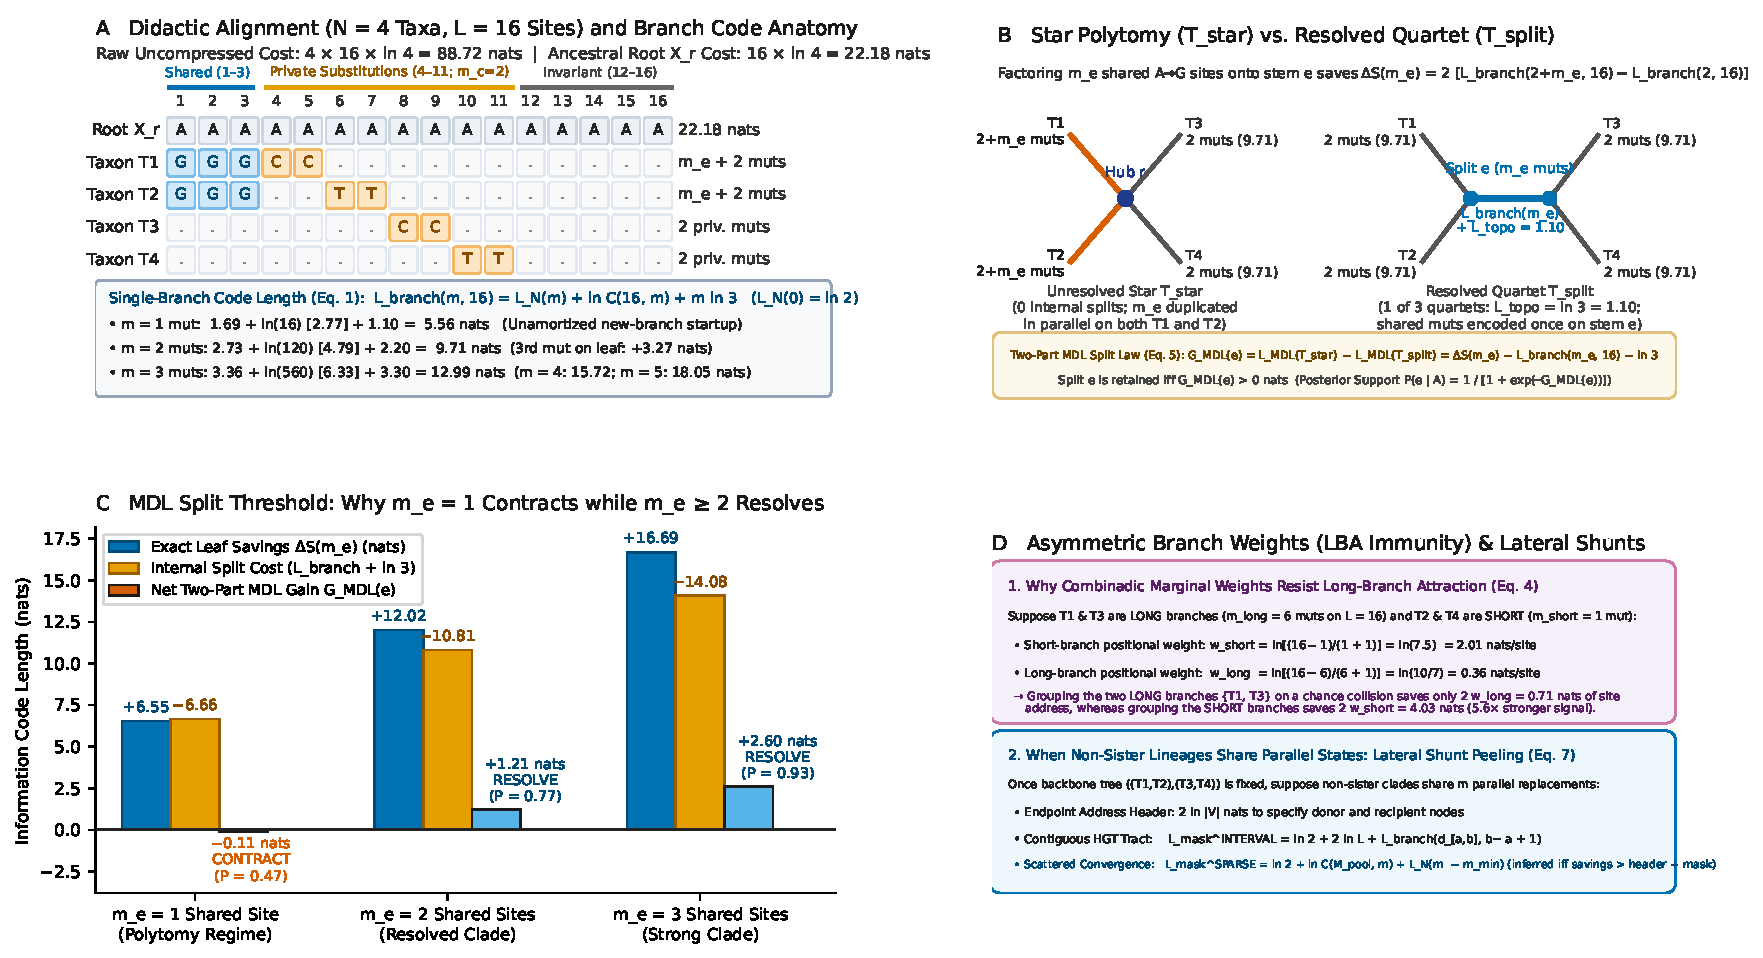
\includegraphics[width=0.95\textwidth]{fig_didactic_mdl.pdf}
\caption{\textbf{Worked two-part MDL ledger on a 4-taxon, 16-site alignment ($N = 4, L = 16$).} (\textbf{A}) Alignment matrix ($X_r = \texttt{A}^{16}$, $88.72\text{ nats}$ raw, $22.18\text{ nats}$ root) and single-branch code lengths $\mathcal{L}_{\text{branch}}(m, 16) = 5.56, 9.71, 12.99\text{ nats}$ ($m = 1, 2, 3$) from Eq.~\eqref{eq:branch_code}. (\textbf{B}) Unresolved star baseline $T_{\text{star}}$ ($61.02\text{ nats}$) versus resolved quartet ($\mathcal{L}_{\text{topo}}(2,2) = \ln 3 = 1.10\text{ nats}$; $75.11\text{ nats}$ total at $m_e = 3$). (\textbf{C}) Exact leaf savings $\Delta\mathcal{L}_{\text{children}}(m_e)$, split cost, and net gain $G_{\text{MDL}}(e)$ for $m_e = 1$ ($-0.11\text{ nats}, P_{\text{local}} = 0.47$, contracted), $m_e = 2$ ($+1.21\text{ nats}, P_{\text{local}} = 0.77$), and $m_e = 3$ ($+2.60\text{ nats}, P_{\text{local}} = 0.93$). (\textbf{D}) Combinadic positional asymmetry ($w_{\text{short}} = 2.01$ vs.\ $w_{\text{long}} = 0.36\text{ nats}$) and Eq.~\eqref{eq:shunt_masks} shunt pricing.}
\label{fig:supp_didactic}
\end{figure}

\begin{figure}[H]
\centering
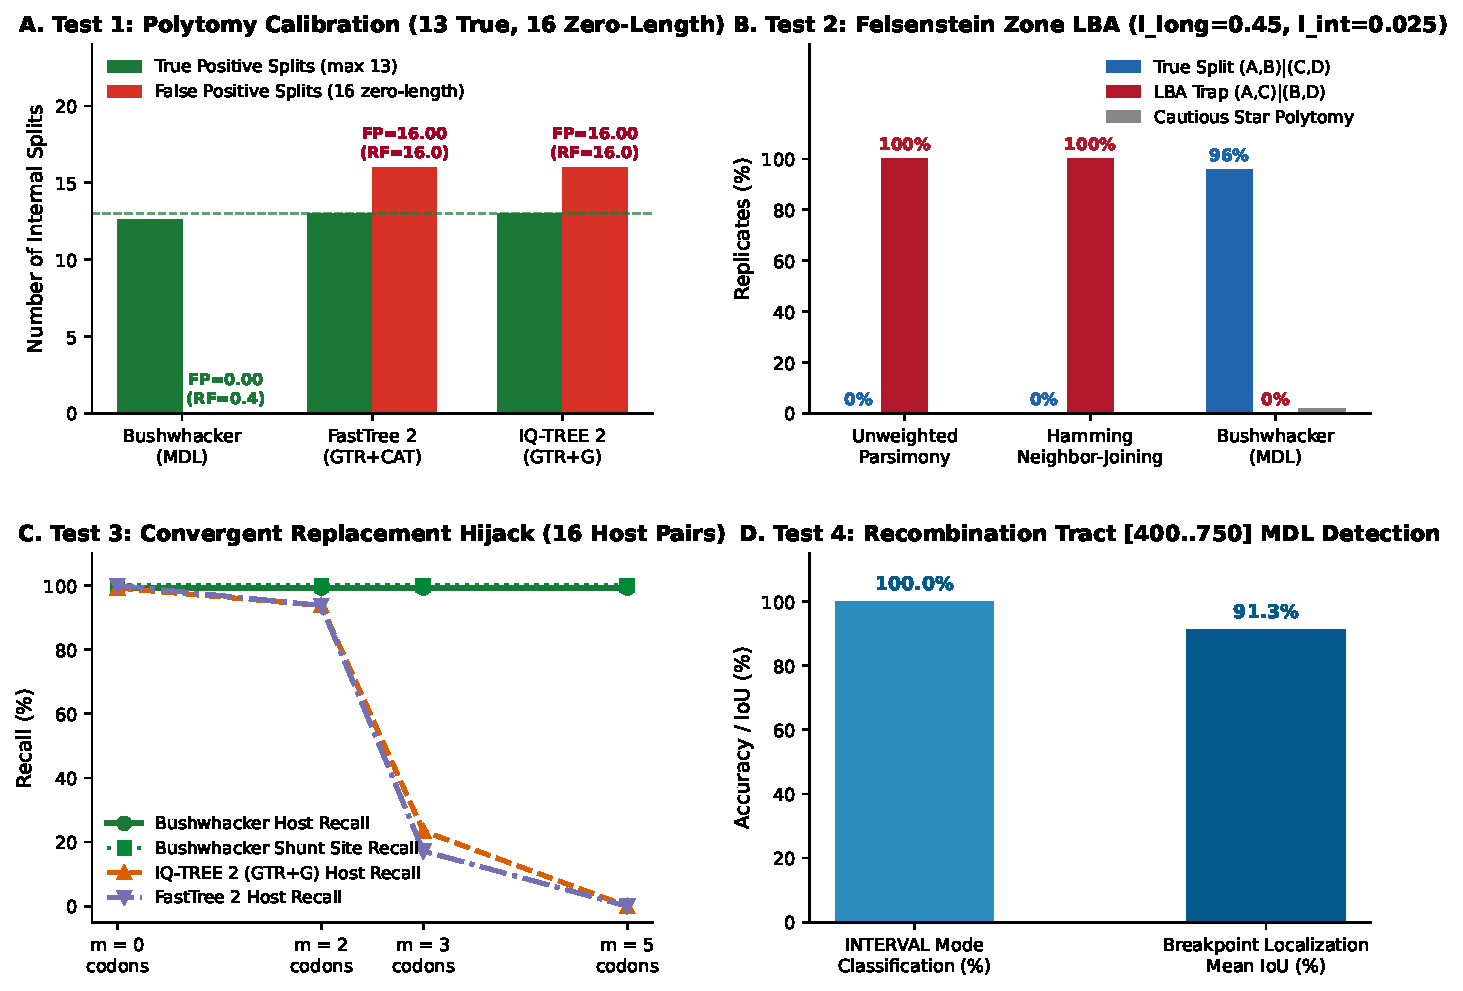
\includegraphics[width=0.95\textwidth]{fig1_synthetic_benchmarks.pdf}
\caption{\textbf{Ground-truth control benchmarks across polytomy calibration, Felsenstein long-branch attraction, convergent hijack, and recombination tracts.} (\textbf{A}) Polytomy test ($13$ true and $16$ zero-length internal splits): Bushwhacker emits $0.00$ false splits ($\text{RF} = 0.4$) versus $16.00$ false splits under forced-binary \texttt{FastTree 2} and \texttt{IQ-TREE 2}. (\textbf{B}) Felsenstein Zone ($l_{\text{long}} = 0.45$, $l_{\text{int}} = 0.025$): $96\%$ true split recovery and $0\%$ long-branch attraction versus $100\%$ attraction under unweighted parsimony and neighbor-joining. (\textbf{C}) Sister-clade preservation across $m = 0 \to 5$ convergent codons ($16$ host pairs; $99.2\%$ Bushwhacker recall versus $0\%$ binary ML recall at $m=5$). (\textbf{D}) Exact \texttt{INTERVAL} classification ($100.0\%$) and breakpoint localization ($\text{IoU} = 91.3\%$) on $[400, 750]$ mosaic tracts.}
\label{fig:supp_synthetic}
\end{figure}

\begin{figure}[H]
\centering
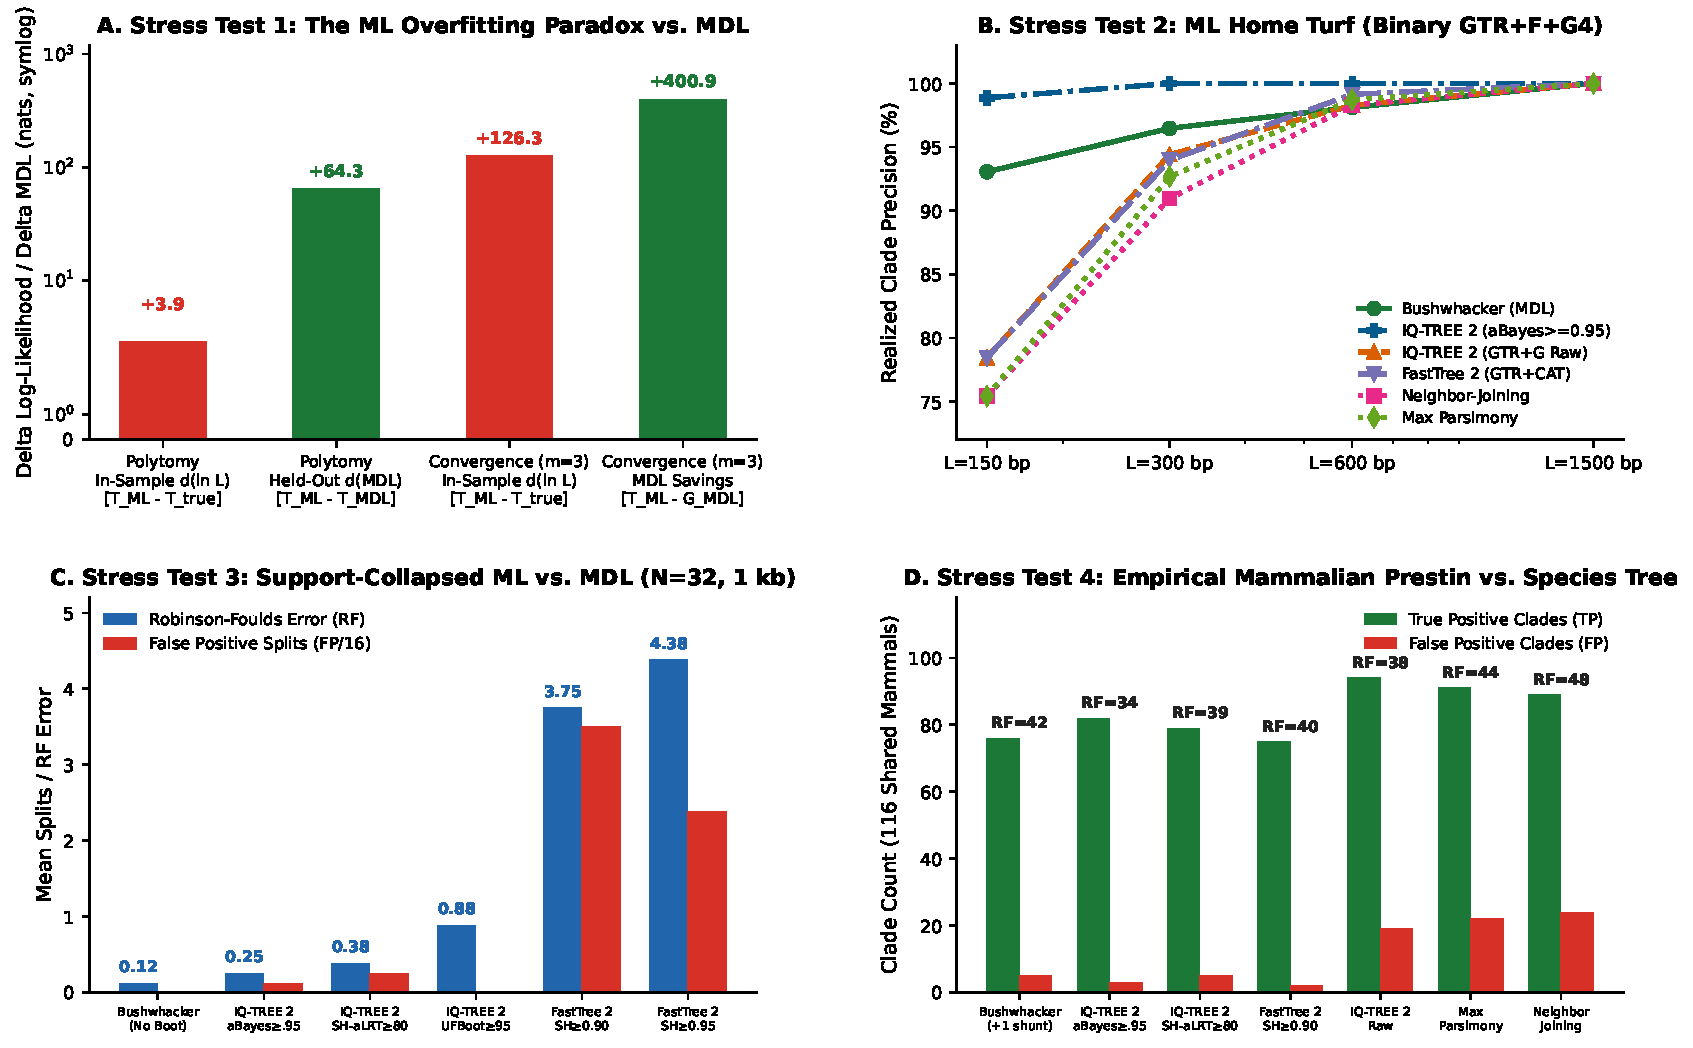
\includegraphics[width=0.95\textwidth]{fig3_stress_tests.pdf}
\caption{\textbf{Overfitting controls, support-collapsed baselines, and empirical mammalian \textit{Prestin} comparison.} (\textbf{A}) In-sample binary ML likelihood excess ($+3.90$ and $+126.3\text{ nats}$) versus out-of-sample held-out compression advantage ($+64.3\text{ nats}$ on multifurcations; $+400.9\text{ nats}$ under $m=3$ convergence). (\textbf{B}) Realized clade precision on strictly binary \texttt{GTR+F+G4} trees across $L = 150 \to 1,500\text{ bp}$. (\textbf{C}) Mean RF error and false splits for Bushwhacker ($0.12\text{ RF}$) versus \texttt{IQ-TREE 2} (\texttt{aBayes}, \texttt{SH-aLRT}, \texttt{UFBoot}) and \texttt{FastTree SH} cutoffs. (\textbf{D}) Empirical $116$-mammal \textit{Prestin} split recovery relative to the NCBI mammalian species tree (all $116$ taxa; $76\text{ TP}, 5\text{ FP}, 93.8\%$ precision under Bushwhacker with $+1$ echolocation shunt).}
\label{fig:supp_stress}
\end{figure}

\begin{figure}[H]
\centering
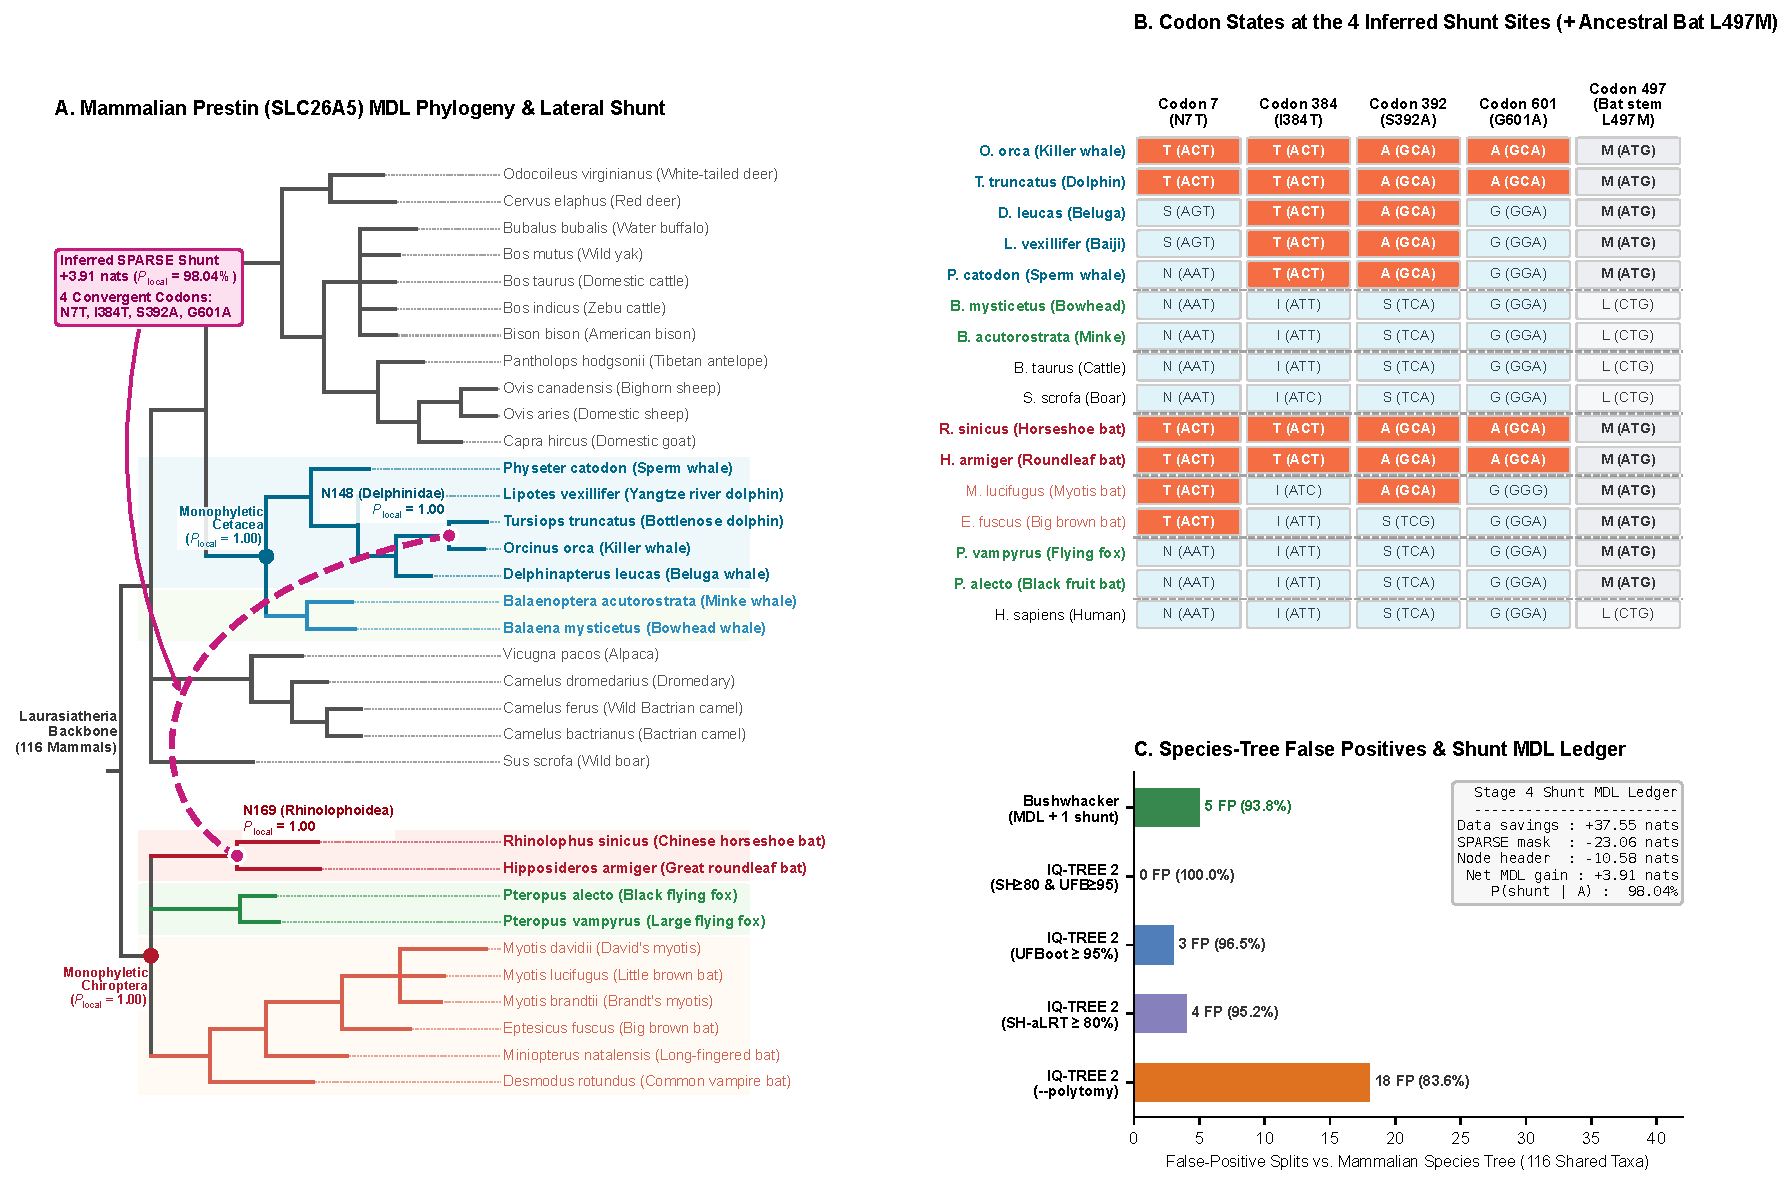
\includegraphics[width=0.95\textwidth]{fig_prestin_convergence.pdf}
\caption{\textbf{Unsupervised graph induction on 116-mammal \textit{Prestin} (\texttt{SLC26A5}) preserves cetacean and bat monophyly while isolating convergent echolocation codons.} (\textbf{A}) Laurasiatheria subtree showing monophyletic Cetacea within Artiodactyla ($P_{\text{local}}=1.00$), monophyletic Chiroptera ($P_{\text{local}}=1.00$), and the \texttt{SPARSE} lateral link ($+3.91\text{ nats}, P_{\text{local}} = 98.04\%$) uniting Delphinidae and Rhinolophoidea bats across codons \texttt{7, 384, 392, 601}. (\textbf{B}) Codon and amino-acid states across the four classic echolocation sites (\texttt{N7T}, \texttt{I384T}, \texttt{S392A}, \texttt{G601A}), contrasted with Chiroptera stem substitution \texttt{L497M} shared by non-echolocating \textit{Pteropus} fruit bats. (\textbf{C}) False-positive species-tree splits across inference methods ($5\text{ FP}, 93.8\%$ precision for Bushwhacker vs.\ $3\text{ FP}/96.5\%$ \texttt{IQ-TREE UFBoot95}, $4\text{ FP}/95.2\%$ \texttt{SH-aLRT80}, $18\text{ FP}/83.6\%$ \texttt{--polytomy}, and $19\text{ FP}/83.2\%$ raw \texttt{IQ-TREE 2} [$78.9\text{ s}$]) and exact two-part MDL shunt ledger.}
\label{fig:supp_prestin}
\end{figure}

\begin{figure}[H]
\centering
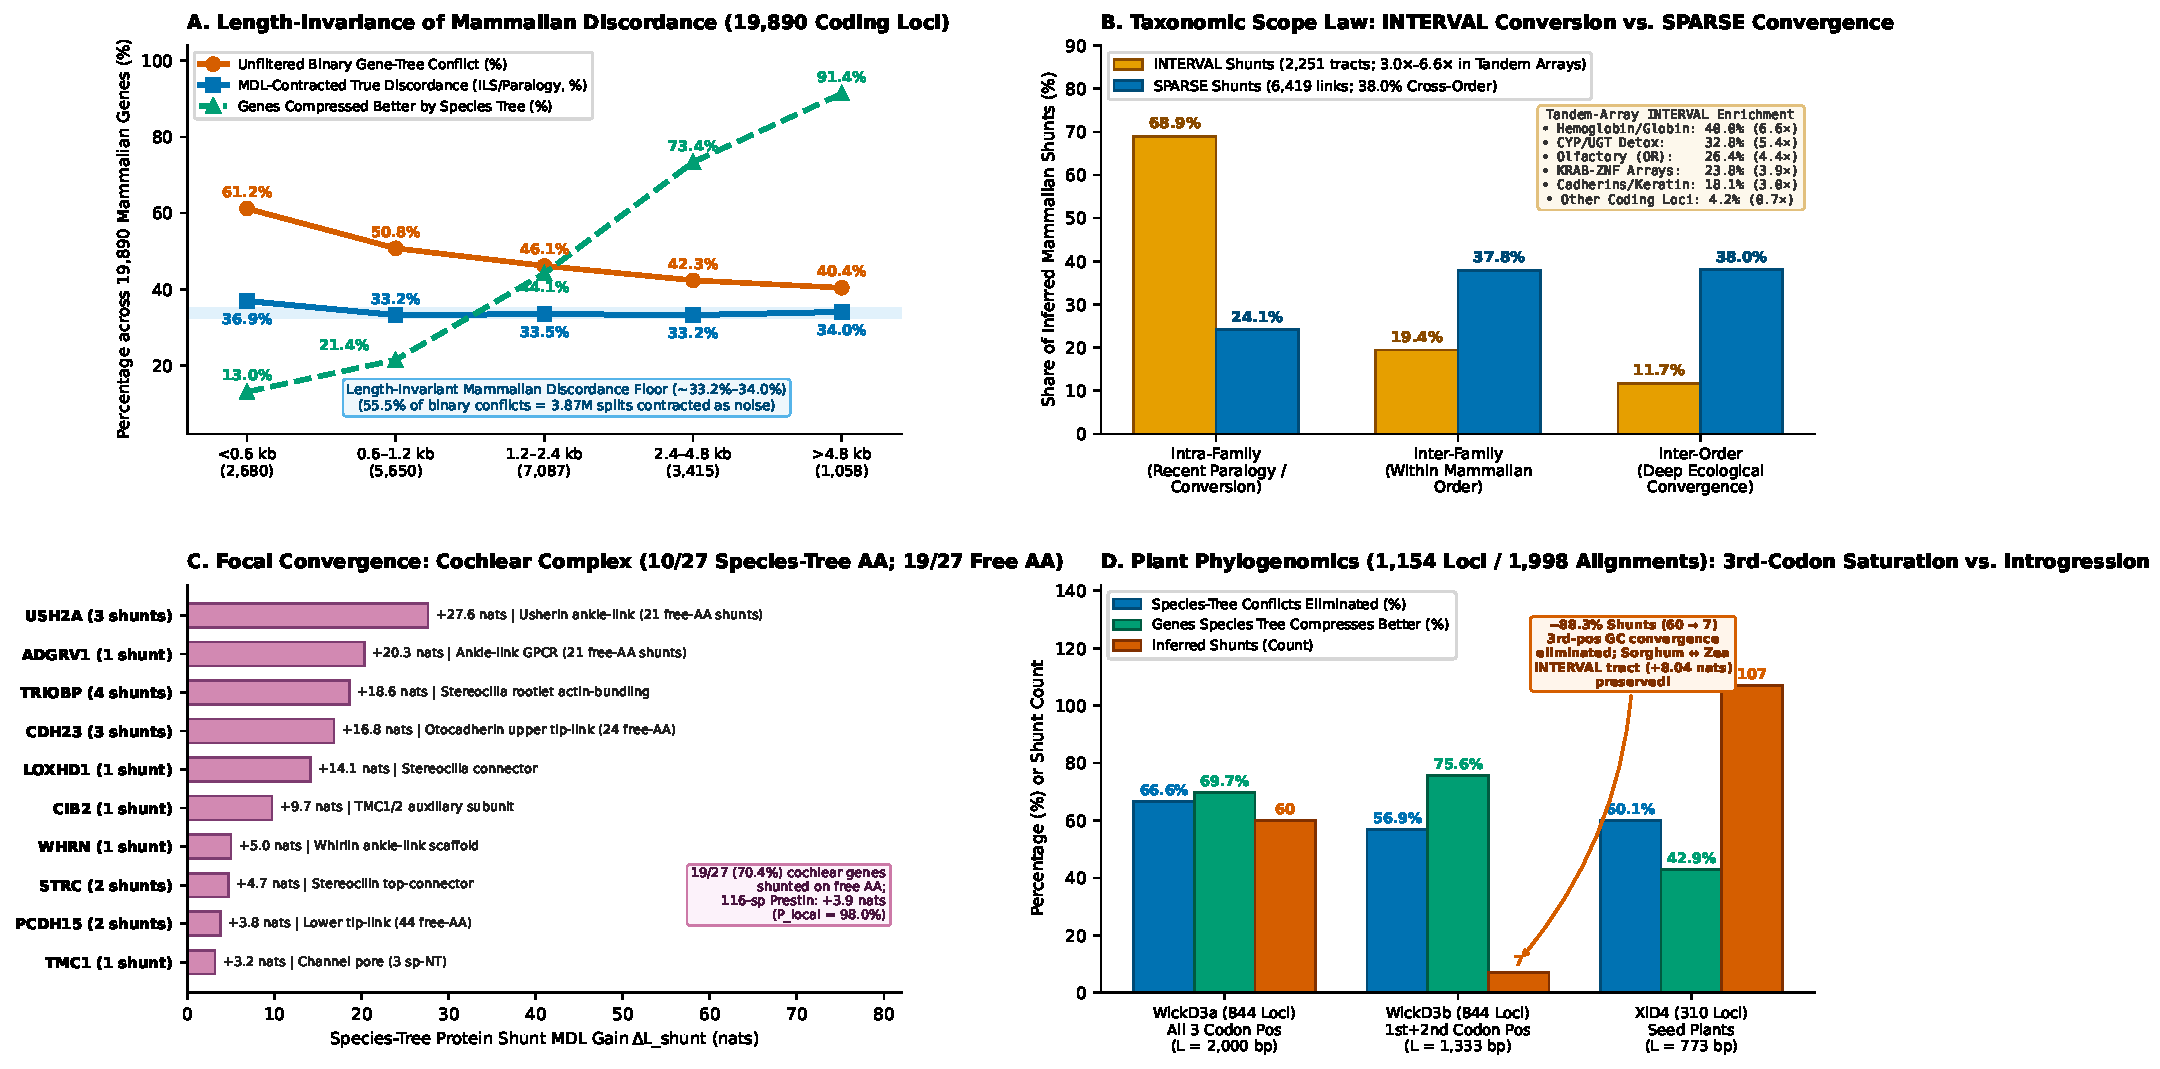
\includegraphics[width=0.95\textwidth]{fig_kingdom_synthesis.pdf}
\caption{\textbf{Mammalian coding-DNA discordance floor, paralog conversion versus cross-order convergence, cochlear co-convergence, and land-plant saturation.} (\textbf{A}) Length stratification across $19,952$ TOGA2 coding genes showing $55.5\%$ ($3.87\text{ million}$) conflict removal down to a $\sim 33.2\text{--}34.0\%$ genealogical floor. (\textbf{B}) Taxonomic scope across $8,670$ species-tree 20-state AA shunts separating contiguous block conversion ($2,251$ tracts; $68.9\%$ intra-family, $3.0\text{--}6.6\times$ enriched in tandem/multicopy families vs.\ $4.2\%$ background) from scattered parallel links ($6,419$ events; $38.0\%$ cross-order). (\textbf{C}) Species-tree 20-state AA shunt gains across the $10/27$ shunted core cochlear hair-cell proteins (\texttt{USH2A} $+27.6\text{ nats}$, \texttt{ADGRV1} $+20.3\text{ nats}$, \texttt{TRIOBP} $+18.6\text{ nats}$, \texttt{CDH23} $+16.8\text{ nats}$, \texttt{LOXHD1} $+14.1\text{ nats}$; $19/27$ in free-tree AA; $116$-mammal coding \textit{Prestin} $+3.91\text{ nats}$). (\textbf{D}) Land-plant all-codon (\texttt{WickD3a}) versus codons $1+2$ (\texttt{WickD3b}) eliminating $88.3\%$ ($60 \to 7$) of GC/AT artifacts while keeping \textit{Sorghum}--\textit{Zea} conversion ($+8.04\text{ nats}$).}
\label{fig:supp_kingdom}
\end{figure}

\begin{figure}[H]
\centering
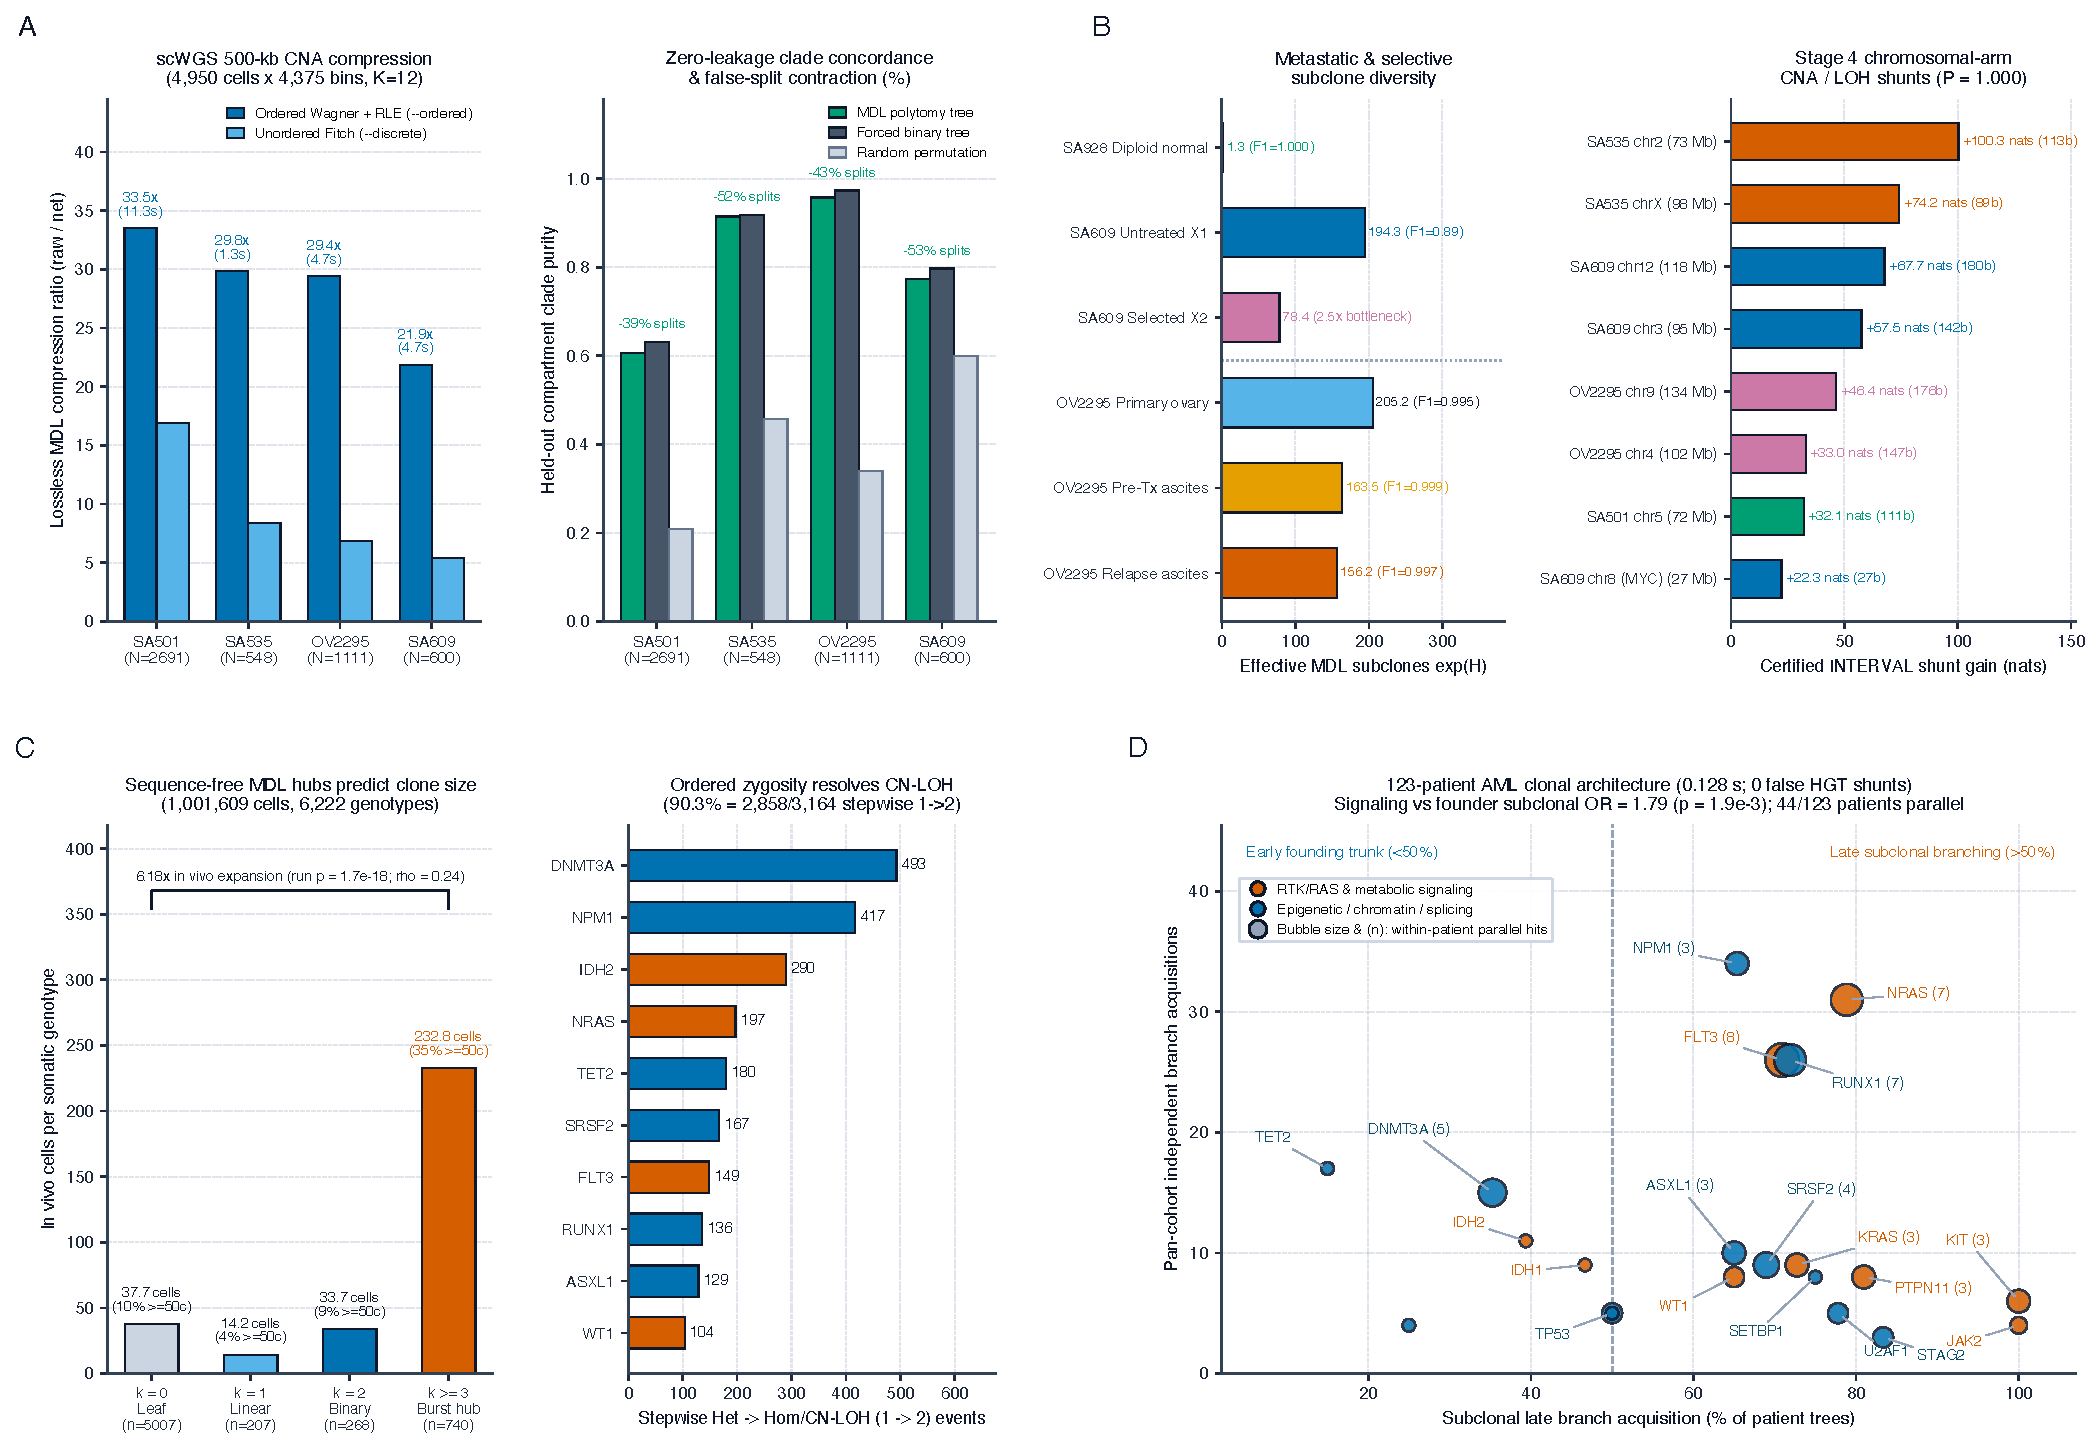
\includegraphics[width=0.95\textwidth]{fig_science_cancer_singlecell.pdf}
\caption{\textbf{Zero-leakage single-cell cancer phylogenomics across 4,950 DLP+ whole-genome copy-number profiles and 1,001,609 myeloid cells.} (\textbf{A}) Ordered 12-state copy-number compression ($21.9\text{--}33.5\times$ raw bins across \texttt{SA501}, \texttt{SA535}, \texttt{OV2295}, \texttt{SA609}) alongside held-out anatomic/passage clade purity (\texttt{OV2295} $95.7\%$ purity, $F_1 = 0.997$ seg / $0.995$ bin) and $33.1\text{--}49.9\%$ ($39.0\text{--}53.1\%$ segments) false-split contraction. (\textbf{B}) Subclonal diversity bottlenecks and inferred chromosomal-arm CNA/LOH tracts including \texttt{MYC} and \texttt{TP53}. (\textbf{C}) Across $168$ Tapestri myeloid runs ($1,001,609$ cells, $6,222$ clones \cite{sollier2023compass}), inferred hub out-degree $k \ge 3$ predicts $6.18\times$ larger in vivo clone sizes (per-run Wilcoxon $p = 1.7\times 10^{-18}, q = 1.7\times 10^{-17}$; $\rho = 0.24$) and captures $90.3\%$ ($2,858/3,164$) stepwise $\text{WT}\to\text{HET}\to\text{HOM}$ CN-LOH transitions. (\textbf{D}) Trunk-versus-subclone driver landscape across $123$ AML patients \cite{morita2020clonal} ($\text{OR} = 1.79$ late signaling enrichment, $p = 1.9\times 10^{-3}, q = 2.8\times 10^{-3}$; parallel acquisitions in $44$ patients).}
\label{fig:supp_cancer}
\end{figure}

\clearpage

\begin{figure}[H]
\centering
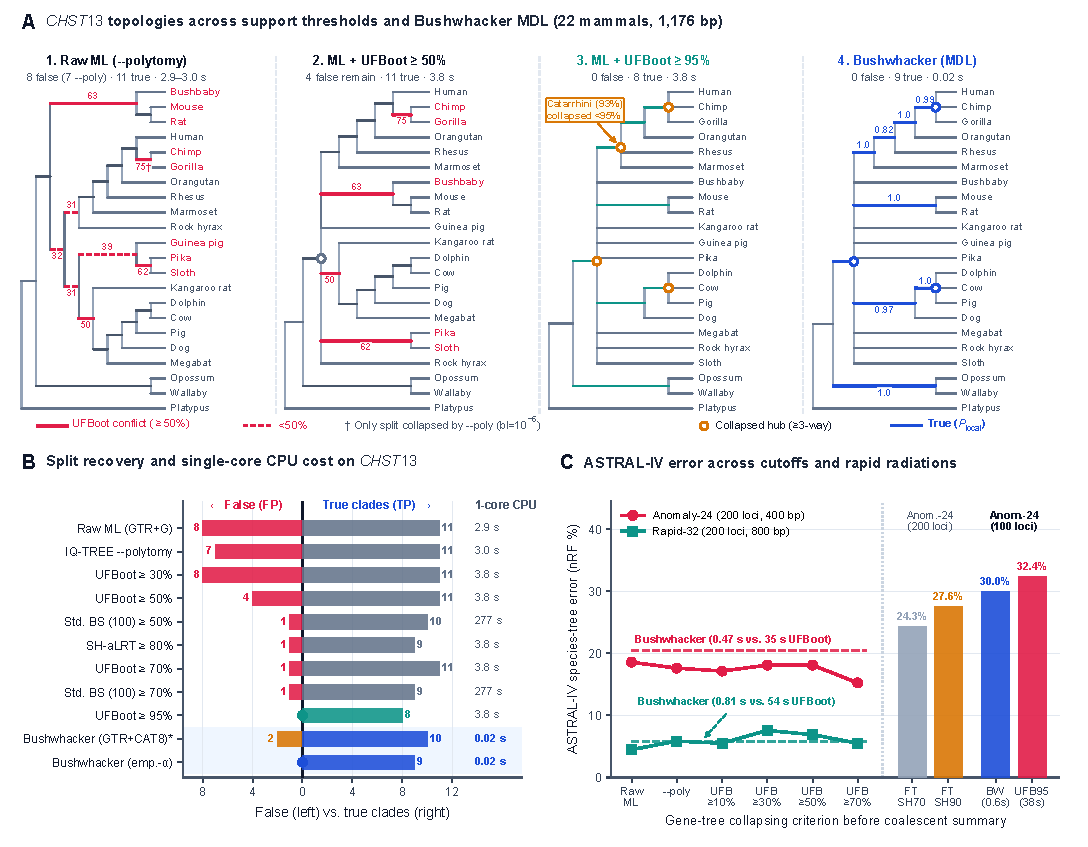
\includegraphics[width=0.96\textwidth]{fig_supp_chst13_bootstrap.pdf}
\caption{\textbf{Support-thresholded maximum likelihood versus deterministic MDL contraction on mammalian \textit{CHST13} and multi-locus \texttt{ASTRAL-IV} radiations.} (\textbf{A}) Side-by-side cladograms on the $22$-mammal \textit{CHST13} alignment ($1,176\text{ bp}$; main-text Fig.~3A) comparing raw \texttt{IQ-TREE} (\texttt{GTR+G}, $8$ false splits in crimson; \texttt{{-}{-}polytomy} removes only \texttt{Gorilla+Chimp}, $\mathrm{bl}=10^{-6}$, marked $\dagger$), \texttt{UFBoot} $\ge 50\%$ ($4$ conflicts remain at $50\text{--}75\%$), \texttt{UFBoot} $\ge 95\%$ ($0$ conflicts, but collapses true \texttt{Catarrhini} [$93\%$] into an amber polytomy alongside \texttt{Dolphin+Cow} [$91\%$]), and Bushwhacker (\texttt{{-}{-}empirical-alpha}, $0$ conflicts, $9$ true clades at $P_{\text{local}}=0.82\text{--}1.00$ in $0.02\text{ s}$). (\textbf{B}) Precision--recall--runtime frontier across ML collapsing rules (\texttt{1}-core CPU, including $100$-replicate nonparametric bootstrap at $277\text{ s}$); asterisk marks default \texttt{GTR+CAT8} ($10$ TP, plus $2$ borderline splits at $P_{\text{local}}=0.664\text{--}0.690$ and $0$ FP for $P_{\text{local}} \ge 0.74$, $0.02\text{ s}$). (\textbf{C}) Multi-locus \texttt{ASTRAL-IV} species-tree error ($\mathrm{nRF}\,\%$) across \texttt{UFBoot} collapse cutoffs on $200$-locus \texttt{Anomaly-24} ($400\text{ bp}$) and \texttt{Rapid-32} ($800\text{ bp}$) simulations ($0.47\text{--}0.81\text{ s}$ Bushwhacker vs.\ $35\text{--}54\text{ s}$ \texttt{UFBoot} on $64$ cores), contrasted on the right with \texttt{FastTree SH90} ($27.6\%$) and $100$-locus \texttt{Anomaly-24} \texttt{UFBoot} $\ge 95\%$ ($32.4\%$ vs.\ $30.0\%$ Bushwhacker).}
\label{fig:supp_chst13_bootstrap}
\end{figure}

\clearpage
% ============================================================================
\section*{Supplementary Tables}
% ============================================================================

\begin{table}[H]
\centering
\caption{\textbf{Master overview of empirical biological corpora and ground-truth simulation suites evaluated with Bushwhacker.} All single-cell abundance counts, DMS binding affinities, clinical timepoints, and taxonomic labels were strictly withheld during tree and network inference.}
\label{tab:master_corpora}
\scriptsize
\setlength{\tabcolsep}{4pt}
\resizebox{\textwidth}{!}{%
\begin{tabular}{@{}llrrll@{}}
\toprule
Biological Scale / Benchmark Suite & Alphabet / Mode & Datasets / Runs & Taxa or Cells ($\times L$) & Primary Biological / Statistical Target & Key Finding \\
\midrule
Model-Selection Archive \cite{abadi2019model,gerth2019cannot} & Nucleotide (4-state) & $7,200$ & $7\text{--}150 \times 100\text{--}8{,}000\text{ bp}$ & BIC vs.\ GTR+I+G4 vs.\ JC discordance & $96.4\%$ of model-conflicting splits contracted \\
Eukaryotic Radiations \cite{shen2017contentious,zhou2018evaluating,shultz2019widespread} & NT \& 20-state AA & $45,255$ ($45,205 + 50$ avian; $11,164$ \texttt{ASTER}) & $20$ corpora ($19 + 1$; $83,180$ ML runs) & Gene-tree conflict \& \texttt{ASTRAL-IV} & $94.5\%$ search-unstable \& $61.5\%$ sp.\ conflict cut \\
Mammalian Proteome (TOGA2 \cite{malovichko2026toga2}) & Codon NT \& 20-state AA & $39,905$ ($19,952\text{ NT} + 19,953\text{ AA}$) & Up to $882$ sp.\ ($20$ orders) & Species concordance, conversion, convergence & $72.7\%$ AA conflict cut; $3.0\text{--}6.6\times$ conversion; $1.35\times$ len-adj.\ guilds \\
Mammalian Supermatrix \cite{malovichko2026toga2} & GTR+CAT8 \& LG08+CAT8 & $2$ ($253$ loci) & $882 \times 543{,}864\text{ bp} / 181{,}288\text{ AA}$ & Deep mammalian Tree of Life & $92.7\%$ IQ-TREE agreement; $24\text{--}37\times$ faster ($193\text{--}288\times$ FT) \\
Prokaryotic Domains (GTDB r95 \cite{parks2020gtdb}) & NT, AA, \& LG08+CAT8 & $434$ + $2$ supermatrices & $1,672$ Archaea; $1,000$ Bacteria & Precambrian phyla \& Complexity Hypothesis & $82.4\text{--}94.3\%$ phyla; $11.8\%$ vs.\ $0\%$ \texttt{ar122} HGT ($p=0.213$) \\
Botanical \& Poaceae $\text{C}_4$ \cite{wickett2014phylotranscriptomic,christin2012adaptive} & Codon NT \& 20-state AA & $2,002$ & Up to $483$ plant species & 3rd-codon GC/AT bias \& $\text{C}_4$ HGT + conv. & $88.3\%$ 3rd-pos.\ shunts removed; $\text{C}_4$ HGT+conv. \\
Clinical \textit{K.\ pneumoniae} \cite{wyres2020population} & NT \& 20-state AA & $9\text{--}16$ str.; $222$ loci & $9\text{--}16$ genomes ($214\text{ kb} + \textit{blaKPC}$) & Chromosomal core vs.\ resistance plasmid & $99.5\%$ vertical core vs.\ $83.3\%$ star plasmid \\
Pandemic Viruses (SARS-CoV-2, DENV, HIV) & NT, AA, \& \texttt{.bwz} & $16$ cohorts & $10,062$ SC2; $5,498$ DENV-1..4 & Superspreading hubs, recombinants, \texttt{.bwz} & $38.5\text{ B}$ payload / $63.2\text{ B}$ arch.\ ($18.9\times$/$11.5\times$ gzip); $76{,}000\times$ GARD \\
Microbiome 16S rRNA \cite{mcdonald2012greengenes} & Nucleotide \& \texttt{.bwz} & $8$ scaling tiers & $256 \to 32,768 \times 1{,}348\text{ bp}$ & Single-marker topological saturation & $91.4\% \to 76.0\%$ supported; $4.5\text{--}11.9\times$ FastTreeMP \\
Germinal-Center B Cells \cite{tas2016visualizing,dewitt2026gcreplay} & Nucleotide (deduplicated) & $148$ GCs ($147+1$) & $10,495$ B cells ($9,394$ geno.) & In vivo clonal bursts \& DMS $K_D$ affinity & $9.5\times$ expansion ($p=5.9\times 10^{-6}$); FE OLS $p=5.3\times 10^{-10}$ \\
Human Myeloid scDNA \cite{morita2020clonal,sollier2023compass} & Ordered 3-state zygosity & $291$ ($168$ runs + $123$ pts) & $1,001,609$ cells ($6,222$ clones) & Leukemic expansion, CN-LOH, late signaling & $6.18\times$ hub cells ($p=1.7\times 10^{-18}$); FE $p=1.4\times 10^{-28}$; $90.3\%$ LOH \\
Human Tumor DLP+ scWGS \cite{salehi2023sitka} & Ordered 12-state CNA & $4$ cohorts (seg + bin) & $4,950$ cells $\times 4{,}375$ $500\text{-kb}$ bins & Subclonal aneuploidy \& ascites evolution & $21.9\text{ s}$ seg ($21.9\text{--}33.5\times$ comp.); $F_1 = 0.997$ purity \\
Ground-Truth Simulations \cite{lytrong2022alisim,abadi2019model} & NT, AA, MSC, Net, Somatic & $36,920$ (+ $100$ GCs) & $7\text{--}1{,}024$ taxa; $L = 40\text{--}16{,}000$ & Polytomies, calibration, HGT, single-cell & $99.7\text{--}100\%$ burst prec.; $3.73\%$ ECE; $0\%$ HGT FPR \\
\bottomrule
\end{tabular}%
}
\end{table}

\begin{table}[H]
\centering
\caption{\textbf{Multi-alphabet ground-truth validation across 20-state proteins, Anomaly-Zone multi-species coalescence, reticulate networks, and single-cell somatic profiles ($9,300$ histories; complementing the $27,720$ nucleotide alignments in Tables~S4 and S5).}}
\label{tab:multialphabet_sim}
\scriptsize
\setlength{\tabcolsep}{4.2pt}
\resizebox{\textwidth}{!}{%
\begin{tabular}{@{}llcccccc@{}}
\toprule
Suite \& Ground-Truth Regime & Method / Configuration & Res / True & FP / Tree & Precision & Recall & nRF / Auxiliary Metric & Time (s) \\
\midrule
\textbf{Protein Suite} (\texttt{LG+G4}, $N=64, L=400\text{ AA}$) & & & & & & & \\
\texttt{P1} Star Burst ($100$ reps, $0$ true splits) & Bushwhacker (\texttt{--protein} MDL) & $0.05 / 0.0$ & $0.05$ & $96.0\%$ (0-FP) & --- & $0.08\%$ FPR & $0.81$ \\
& IQ-TREE 2 (\texttt{LG+G4 --polytomy}) & $38.67 / 0.0$ & $38.67$ & $0.0\%$ & --- & $63.4\%$ FPR & $9.08$ \\
& IQ-TREE 2 / FastTree 2 (Binary) & $61.00 / 0.0$ & $61.00$ & $0.0\%$ & --- & $100.0\%$ FPR & $9.11 / 4.59$ \\
\texttt{P2} Rapid Radiation ($50\%$ silent stems) & Bushwhacker (\texttt{--protein} MDL) & $30.14 / 30.49$ & $0.05$ & $99.8\%$ & $98.6\%$ & $\text{nRF} = 0.0077$ & $1.39$ \\
& IQ-TREE 2 (\texttt{--polytomy}) & $50.31 / 30.49$ & $19.84$ & $60.5\%$ & $99.9\%$ & $\text{nRF} = 0.3362$ & $8.06$ \\
& IQ-TREE 2 / FastTree 2 (Binary) & $61.00 / 30.49$ & $30.55 / 30.54$ & $49.9\%$ & $99.9\%$ & $\text{nRF} = 0.5189$ & $8.01 / 3.84$ \\
\texttt{P3} Standard Resolved Yule ($61$ splits) & Bushwhacker (\texttt{--protein} MDL) & $59.60 / 61.0$ & $0.01$ & $100.0\%$ & $97.7\%$ & $\text{nRF} = 0.0116$ & $0.99$ \\
& IQ-TREE 2 (\texttt{LG+G4}) & $61.00 / 61.0$ & $0.08$ & $99.9\%$ & $99.9\%$ & $\text{nRF} = 0.0013$ & $7.04$ \\
\texttt{P4} Convergent Protein Sites ($45$ splits) & Bushwhacker (\texttt{--protein} + Stage 4) & $44.40 / 45.0$ & $0.01$ & $100.0\%$ & $98.6\%$ & $92.8\%$ conv.\ AA site prec.; $0\%$ false clade & $0.89$ \\
\midrule
\textbf{Coalescent MSC \& B-Cell GC Suite} ($8,100$ trees) & & & & & & & \\
24-sp.\ Asymmetric Anomaly Zone ($L=400\text{ bp}$) & Bushwhacker (MDL) $\to$ ASTRAL-IV & $37.8\%$ gene res. & --- & --- & --- & Species $\text{nRF} = 0.2048$ ($-15.6\%$ vs.\ FT) & $0.47$ \\
& FastTree 2 (raw / SH-collapsed) $\to$ ASTRAL & $100\%$ / SH & --- & --- & --- & Species $\text{nRF} = 0.2429\text{--}0.2762$ & $2.10$ \\
32-sp.\ Rapid Radiation ($L=800\text{ bp}$) & Bushwhacker (MDL) $\to$ ASTRAL-IV & $54.1\%$ gene res. & --- & --- & --- & Species $\text{nRF} = 0.0586$ (ties IQ \texttt{--poly}) & $0.62$ \\
50-Galton--Watson B-Cell GCs ($90$ cells/GC) & Bushwhacker (MDL) & $7.34 / 35.26$ & $0.02$ & $99.8\%$ & $20.7\%$ & $F_1 = 0.3356$ ($0.7533$ cell); burst $\rho = 0.438$ & $0.10$ \\
& \texttt{GCtree} (zero-leakage / abund.-oracle) & $38.10 / 37.86$ & $5.96 / 5.62$ & $84.4\% / 85.2\%$ & $91.2\% / 91.4\%$ & Unique geno.\ $F_1 = 0.8760 / 0.8813$ & $11.62 / 11.87$ \\
50 Neutral B-Cell GCs ($\beta_{\text{bind}} = 0$ control) & Bushwhacker (MDL) & $8.58 / 33.92$ & $0.04$ & $99.5\%$ & $25.1\%$ & Null paired hub abund.\ $p=0.705$, affin.\ $p=0.833$ & $0.05$ \\
\midrule
\textbf{Reticulate Network Suite} ($400$ sims, $45$ splits) & & & & & & & \\
\texttt{N1} Strictly Clonal Null ($100$ + $200$ AliSim) & Bushwhacker (MDL + Stage 4) & $44.98 / 45.0$ & $0.00$ & $100.0\%$ & $99.96\%$ & $0.0\%$ false lateral shunts ($100\%$ spec.) & $0.09$ \\
\texttt{N2} Short Contiguous HGT ($200\text{ bp}$) & Bushwhacker (MDL + Stage 4) & $44.96 / 45.0$ & $0.09$ & $99.8\%$ & $99.7\%$ & $37.0\%$ \texttt{INTERVAL} ($\text{IoU} = 0.274$; $0\%$ false clade) & $0.11$ \\
\texttt{N3} Contiguous HGT Tract ($450\text{ bp}$) & Bushwhacker (MDL + Stage 4) & $44.94 / 45.0$ & $1.34$ & $97.0\%$ & $96.9\%$ & $90.0\%$ \texttt{INTERVAL} ($\text{IoU} = 0.715$; $0\%$ false clade) & $0.12$ \\
\texttt{N4} Scattered Convergence ($10$ NT sites) & Bushwhacker (MDL + Stage 4) & $44.95 / 45.0$ & $0.00$ & $100.0\%$ & $99.9\%$ & $92.0\%$ \texttt{SPARSE}; $99.2\%$ site prec.; $90.9\%$ rec. & $0.10$ \\
\midrule
\textbf{Single-Cell Somatic Suite} ($400$ matrices) & & & & & & & \\
\texttt{C1} Binary SNV Clonal Burst ($5\%$ dropout) & Bushwhacker (\texttt{--discrete} MDL) & $33.34 / 33.47$ & $4.56$ & $86.1\%$ & $85.6\%$ & $6.3\times$ lower FP than binary ML ($\text{nRF}=0.1418$) & $0.035$ \\
& IQ-TREE 2 (Binary \texttt{GTR2/BIN}) & $61.00 / 33.47$ & $28.72$ & $52.9\%$ & $96.4\%$ & $\text{nRF} = 0.4614$ & $0.45$ \\
& \texttt{COMPASS} (MCMC) & $12.90 / 33.47$ & $5.53$ & $57.1\%$ & $22.1\%$ & $\text{nRF} = 0.4733$ & $30.93$ \\
\texttt{C2} High Allelic Dropout ($20\%$ missing) & Bushwhacker (\texttt{--discrete} MDL) & $36.41 / 37.15$ & $13.33$ & $63.2\%$ & $61.9\%$ & $\text{nRF} = 0.3725$ (vs.\ $0.4830$ IQ-TREE BIN) & $0.065$ \\
& \texttt{COMPASS} (MCMC) & $13.70 / 37.15$ & $6.87$ & $49.7\%$ & $18.4\%$ & $\text{nRF} = 0.5011$ & $27.91$ \\
\texttt{C3} Ordered Copy-Number ($K=7$ states $0..6$) & Bushwhacker (\texttt{--ordered} $L_1$ step) & $59.60 / 55.60$ & $5.61$ & $90.6\%$ & $97.1\%$ & $\text{nRF} = 0.0660$ ($46\%$ lower nRF vs.\ binarized) & $0.14$ \\
& Binarized Copy-Number Baseline & $52.37 / 55.60$ & $5.15$ & $90.1\%$ & $84.9\%$ & $\text{nRF} = 0.1224$ ($\text{RF} = 13.53$ vs.\ $7.22$) & $0.14$ \\
\texttt{C4} Noisy Diploid Null ($100$ controls) & Bushwhacker (\texttt{--ordered} MDL) & $0.00 / 0.00$ & $0.00$ & $100.0\%$ & $100.0\%$ & $0.0$ false clones across all $100$ controls & $0.11$ \\
\bottomrule
\end{tabular}%
}
\end{table}

\begin{table}[H]
\centering
\caption{\textbf{Conditional local posterior calibration across $44,337$ inferred branches and $322$ lateral shunts without bootstrap resampling.} Conditional local posterior probability $P_{\text{local}} = (1 + e^{-G_{\text{MDL}}})^{-1}$ is compared directly against ground-truth bipartition membership (Panel~A; mean predicted $P_{\text{local}} = 98.08\%$, empirical true fraction $= 94.35\%$, $\text{ECE} = 3.73\%$) and Stage~4 lateral shunt membership across \texttt{N1--N4} (Panel~B; $322$ shunts, mean predicted $93.57\%$, true $= 90.99\%$, $\text{ECE} = 4.93\%$, with $3$ null shunts across $400$ clonal alignments = $0.0075$/dataset).}
\label{tab:posterior_cal}
\footnotesize
\resizebox{\textwidth}{!}{%
\begin{tabular}{@{}lrrrr@{}}
\toprule
Conditional Local Posterior Bin $P_{\text{local}}(\cdot \mid T_{-\cdot}, A)$ & Features ($n$) & Mean Predicted $P_{\text{local}}$ & Empirical True Fraction & Absolute Gap \\
\midrule
\textbf{Panel A: Internal Tree Branches (Multi-Alphabet)} & & & & \\
$[0.50,\; 0.65)$ & $881$ & $57.60\%$ & $40.64\%$ & $16.96\%$ \\
$[0.65,\; 0.80)$ & $959$ & $72.87\%$ & $48.80\%$ & $24.07\%$ \\
$[0.80,\; 0.90)$ & $807$ & $85.10\%$ & $57.25\%$ & $27.85\%$ \\
$[0.90,\; 0.95)$ & $718$ & $92.65\%$ & $69.36\%$ & $23.29\%$ \\
$[0.95,\; 0.99)$ & $1,353$ & $97.35\%$ & $80.27\%$ & $17.08\%$ \\
$[0.99,\; 1.00]$ & $39,619$ & $99.98\%$ & $98.34\%$ & $1.64\%$ \\
\textbf{Panel A Total / Weighted Summary} & $\mathbf{44,337}$ & $\mathbf{98.08\%}$ & $\mathbf{94.35\%}$ & $\mathbf{ECE = 3.73\%}$ \\
\midrule
\textbf{Panel B: Stage 4 Lateral Shunts (\texttt{N1--N4})} & & & & \\
$[0.50,\; 0.65)$ & $20$ & $57.55\%$ & $75.00\%$ & $17.45\%$ \\
$[0.65,\; 0.80)$ & $20$ & $73.32\%$ & $70.00\%$ & $3.32\%$ \\
$[0.80,\; 0.90)$ & $22$ & $84.26\%$ & $77.27\%$ & $6.99\%$ \\
$[0.90,\; 0.95)$ & $27$ & $92.88\%$ & $88.89\%$ & $3.99\%$ \\
$[0.95,\; 0.99)$ & $47$ & $97.23\%$ & $97.87\%$ & $0.64\%$ \\
$[0.99,\; 1.00]$ & $186$ & $99.90\%$ & $95.16\%$ & $4.74\%$ \\
\textbf{Panel B Total / Weighted Summary ($0.0075$ null shunts/tree)} & $\mathbf{322}$ & $\mathbf{93.57\%}$ & $\mathbf{90.99\%}$ & $\mathbf{ECE = 4.93\%}$ \\
\bottomrule
\end{tabular}%
}
\end{table}

\begin{table}[H]
\centering
\caption{\textbf{Ground-truth accuracy across $27,500$ empirical-parameterized nucleotide histories from published simulation archives \cite{abadi2019model,gerth2019cannot}.} Panel A stratifies \texttt{sim\_bic} ($n = 5,901$) by short ancestral branches ($\ell_e L < 1.0$ expected substitution). Panel B reports homogeneous (\texttt{c0}), site-heterogeneous (\texttt{c1}), and branch-heterogeneous (\texttt{c2}) corpora.}
\label{tab:abadi_gerth}
\scriptsize
\resizebox{\textwidth}{!}{%
\begin{tabular}{@{}llccccccc@{}}
\toprule
Benchmark Stratum & Method & Res / True & $\text{RF}_{\text{bin}}$ & $\text{nRF}_{\text{bin}}$ & $\text{RF}_{\ge 1}$ & $\text{nRF}_{\ge 1}$ & FP / Tree & Precision \\
\midrule
Panel A: \texttt{sim\_bic} All ($n=5,901$) & Bushwhacker (MDL) & $8.9 / 18.1$ & $10.51$ & $0.2727$ & $6.87$ & $0.2303$ & $0.68$ & $94.7\%$ \\
& IQ-TREE 2 (BIC ModelFinder) & $18.1 / 18.1$ & $8.42$ & $0.1666$ & $5.75$ & $0.1616$ & $4.21$ & $83.3\%$ \\
& IQ-TREE 2 ($\text{GTR}+\text{I}+\text{G4}$) & $18.1 / 18.1$ & $8.46$ & $0.1678$ & $5.77$ & $0.1623$ & $4.23$ & $83.2\%$ \\
& IQ-TREE 2 (Jukes--Cantor) & $18.1 / 18.1$ & $8.99$ & $0.1782$ & $6.33$ & $0.1739$ & $4.49$ & $82.2\%$ \\
& IQ-TREE 2 (\texttt{--polytomy}) & $15.4 / 18.1$ & $6.82$ & $0.1404$ & $3.34$ & $0.1147$ & $2.08$ & $89.2\%$ \\
& FastTree 2 & $16.7 / 18.1$ & $7.24$ & $0.1542$ & $4.56$ & $0.1516$ & $2.93$ & $84.9\%$ \\
& BioNJ & $16.7 / 18.1$ & $11.57$ & $0.2642$ & $8.74$ & $0.2710$ & $5.10$ & $73.1\%$ \\
\addlinespace
Low Stemminess ($25\text{--}50\%$ $\ell_e L < 1$, $n=662$) & Bushwhacker (MDL) & $10.7 / 22.0$ & $11.83$ & $0.2744$ & $3.72$ & $0.1522$ & $0.29$ & $98.1\%$ \\
& IQ-TREE 2 (\texttt{--polytomy}) & $14.2 / 22.0$ & $12.05$ & $0.2679$ & $4.38$ & $0.1650$ & $2.14$ & $86.9\%$ \\
& FastTree 2 & $20.5 / 22.0$ & $15.20$ & $0.3306$ & $10.23$ & $0.3150$ & $6.88$ & $68.1\%$ \\
& IQ-TREE 2 (BIC / $\text{GTR}+\text{I}+\text{G4}$) & $22.0 / 22.0$ & $16.51$ & $0.3535$ & $11.57$ & $0.3388$ & $8.26$ & $64.7\%$ \\
\addlinespace
Very Low Stemminess ($>50\%$ $\ell_e L < 1$, $n=625$) & Bushwhacker (MDL) & $7.8 / 33.6$ & $26.14$ & $0.3961$ & $3.69$ & $0.1797$ & $0.18$ & $98.8\%$ \\
& FastTree 2 & $22.3 / 33.6$ & $33.95$ & $0.4992$ & $15.12$ & $0.4964$ & $11.34$ & $51.4\%$ \\
& IQ-TREE 2 (\texttt{--polytomy}) & $20.9 / 33.6$ & $36.27$ & $0.5388$ & $14.20$ & $0.4540$ & $11.79$ & $50.2\%$ \\
& IQ-TREE 2 (BIC / $\text{GTR}+\text{I}+\text{G4}$) & $33.6 / 33.6$ & $45.23$ & $0.6623$ & $26.47$ & $0.6352$ & $22.62$ & $33.8\%$ \\
\midrule
Panel B: \texttt{c0} Homogeneous ($n=7,199$) & Bushwhacker (MDL) & $8.7 / 16.8$ & $13.30$ & $0.3328$ & $9.21$ & $0.3074$ & $2.60$ & $82.5\%$ \\
& IQ-TREE 2 (\texttt{--polytomy} / $\text{GTR}+\text{I}+\text{G4}$) & $14.3 / 16.8$ & $14.70 / 16.43$ & $0.3015 / 0.3337$ & $10.79 / 12.97$ & $0.2865 / 0.3235$ & $6.14 / 8.21$ & $71.6\% / 66.6\%$ \\
\texttt{c1} Site-Heterogeneous ($n=7,200$) & Bushwhacker (MDL) & $8.8 / 16.8$ & $10.19$ & $0.2578$ & $6.11$ & $0.2247$ & $1.09$ & $92.6\%$ \\
& IQ-TREE 2 (\texttt{--polytomy} / $\text{GTR}+\text{I}+\text{G4}$) & $14.2 / 16.8$ & $10.30 / 12.04$ & $0.1843 / 0.2158$ & $6.48 / 8.89$ & $0.1647 / 0.2133$ & $3.85 / 6.02$ & $84.9\% / 78.4\%$ \\
\texttt{c2} Branch-Heterogeneous ($n=7,200$) & Bushwhacker (MDL) & $8.8 / 16.8$ & $10.25$ & $0.2616$ & $6.16$ & $0.2306$ & $1.12$ & $92.4\%$ \\
& IQ-TREE 2 (\texttt{--polytomy} / $\text{GTR}+\text{I}+\text{G4}$) & $14.2 / 16.8$ & $10.36 / 12.08$ & $0.1867 / 0.2180$ & $6.55 / 8.92$ & $0.1682 / 0.2163$ & $3.91 / 6.04$ & $84.6\% / 78.2\%$ \\
\bottomrule
\end{tabular}%
}
\end{table}

\begin{table}[H]
\centering
\caption{\textbf{Worked 4-taxon, 16-site MDL ledger and representative \texttt{AliSim} operating characteristics.} Panel A gives exact nat-by-nat code lengths on a quartet ($N=4, L=16$, $m_c=2$ private leaf edits costing $\mathcal{L}_{\text{branch}}(2,16)=9.71\text{ nats}$ each; matching Fig.~\ref{fig:supp_didactic}). Panel B reports representative \texttt{AliSim} regimes ($10$ replicates each across $22$ scenarios; $220$ alignments total \cite{lytrong2022alisim,robinson1981comparison}).}
\label{tab:synthetic_summary}
\scriptsize
\setlength{\tabcolsep}{4pt}
\resizebox{\textwidth}{!}{%
\begin{tabular}{@{}llcccccc@{}}
\toprule
Panel A: 4-Taxon Quartet Ledger ($L=16$) & Shared Synapomorphies & Leaf Savings $\Delta\mathcal{L}_{\text{children}}$ & Branch Code $\mathcal{L}_{\text{branch}}$ & Topo Cost $\mathcal{L}_{\text{topo}}(2,2)$ & Net Gain $G_{\text{MDL}}(e)$ & Local Post.\ $P_{\text{local}}$ & Decision \\
\midrule
$m_e = 0$ (Zero shared mutations) & $\texttt{. . .} \mid 2\text{ priv.}$ & $0.00\text{ nats}$ & $-0.69\text{ nats}$ & $-1.10\text{ nats}$ & $-1.79\text{ nats}$ & $0.143$ & Contract ($T_{\text{star}}$) \\
$m_e = 1$ (Single shared site) & $\texttt{G . .} \mid 2\text{ priv.}$ & $+6.55\text{ nats}$ & $-5.56\text{ nats}$ & $-1.10\text{ nats}$ & $-0.11\text{ nats}$ & $0.473$ & Contract ($T_{\text{star}}$) \\
$m_e = 2$ (Two shared sites) & $\texttt{G G .} \mid 2\text{ priv.}$ & $+12.02\text{ nats}$ & $-9.71\text{ nats}$ & $-1.10\text{ nats}$ & $+1.21\text{ nats}$ & $0.771$ & Resolve $(\text{T}_1,\text{T}_2)$ \\
$m_e = 3$ (Three shared sites) & $\texttt{G G G} \mid 2\text{ priv.}$ & $+16.69\text{ nats}$ & $-12.99\text{ nats}$ & $-1.10\text{ nats}$ & $+2.60\text{ nats}$ & $0.931$ & Resolve $(\text{T}_1,\text{T}_2)$ \\
\midrule
Panel B: AliSim Regime ($N, L$) & Method & Res / True & FP & Precision & RF & nRF / FPR & Time (s) \\
\midrule
\texttt{S08} Star Null ($128 \times 1{,}000\text{ bp}$) & Bushwhacker (MDL) & $0.0 / 0$ & $0.0$ & $100.0\%$ & $0.0$ & $0.0\%$ FPR & $0.55$ \\
& IQ-TREE 2 (\texttt{--polytomy} / Binary) & $74.8 / 125.0$ & $74.8 / 125.0$ & $0.0\%$ & $74.8 / 125.0$ & $59.8\% / 100\%$ FPR & $482.5 / 391.6$ \\
& FastTree 2 (raw / SH$\ge 0.90$) & $124.6 / 11.9$ & $124.6 / 11.9$ & $0.0\%$ & $124.6 / 11.9$ & $99.7\% / 9.5\%$ FPR & $3.02$ \\
\texttt{S08b} Ultra-Short ($200 \times 100\text{ bp}$) & Bushwhacker (MDL) & $16.3 / 197$ & $0.1$ & $99.7\%$ & $180.9$ & $0.4591$ & $0.37$ \\
& IQ-TREE 2 (\texttt{--polytomy} / Binary) & $142.4 / 197.0$ & $31.3 / 74.0$ & $78.1\% / 62.4\%$ & $117.2 / 148.0$ & $0.2975 / 0.3756$ & $96.2 / 91.1$ \\
\texttt{S10b} Standard ($200 \times 1{,}000\text{ bp}$) & Bushwhacker (MDL / Binary) & $157.2 / 197.0$ & $0.0 / 8.6$ & $100.0\% / 95.6\%$ & $39.8 / 17.2$ & $0.1010 / 0.0437$ & $0.63$ \\
& IQ-TREE 2 (\texttt{--polytomy} / Binary) & $192.8 / 197.0$ & $6.7 / 9.0$ & $96.5\% / 95.4\%$ & $17.6 / 18.0$ & $0.0447 / 0.0457$ & $64.1 / 65.4$ \\
\texttt{S12c} Long Gene ($200 \times 16{,}000\text{ bp}$) & Bushwhacker (MDL) & $196.0 / 197$ & $0.0$ & $100.0\%$ & $1.0$ & $0.0025$ & $2.65$ \\
\texttt{S04} Large Tree ($1{,}024 \times 1{,}000\text{ bp}$) & Bushwhacker (MDL) & $784.9 / 1{,}021$ & $0.1$ & $99.99\%$ & $236.3$ & $0.1157$ & $4.22$ \\
& IQ-TREE 2 (\texttt{--polytomy} / Binary) & $1{,}000.2 / 1{,}021.0$ & $37.4 / 50.1$ & $96.3\% / 95.1\%$ & $95.6 / 100.2$ & $0.0468 / 0.0491$ & $17.6 / 17.9$ \\
& BioNJ \cite{gascuel1997bionj} & $1{,}021.0 / 1{,}021$ & $134.2$ & $86.9\%$ & $268.4$ & $0.1314$ & $0.10$ \\
\texttt{S13} Low-Div Outbreak ($200 \times 1{,}000\text{ bp}$) & Bushwhacker (MDL) & $102.5 / 197$ & $0.0$ & $100.0\%$ & $94.5$ & $0.2398$ & $0.32$ \\
& IQ-TREE 2 (\texttt{--polytomy} / Binary) & $155.6 / 197.0$ & $3.6 / 33.8$ & $97.7\% / 82.8\%$ & $48.6 / 67.6$ & $0.1234 / 0.1716$ & $62.9 / 62.5$ \\
& FastTree 2 & $196.9 / 197$ & $32.9$ & $83.3\%$ & $65.9$ & $0.1673$ & $3.36$ \\
\bottomrule
\end{tabular}%
}
\end{table}

\begin{table}[H]
\centering
\caption{\textbf{Multi-seed maximum-likelihood optimization instability and apparent species-tree conflict removal across eukaryotic phylogenomic radiations.} Top rows report search-unstable ML splits across $20$ independent RAxML/IQ-TREE optimization starts per gene on $4,159$ gene-alignments ($3,315$ unique genes; \texttt{WickD3a}/\texttt{WickD3b} paired codon views) ($83,180$ searches \cite{zhou2018evaluating}). Bottom summary encompasses all $19$ benchmarks ($45,205$ loci \cite{shen2017contentious,zhou2018evaluating}).}
\label{tab:rokas_summary}
\scriptsize
\setlength{\tabcolsep}{4pt}
\resizebox{\textwidth}{!}{%
\begin{tabular}{@{}lccccccc@{}}
\toprule
Dataset ($n_{\text{genes}}$, $\bar{N}$, $\bar{L}$) & Mean $\rho(A)$ & Search-Unstable ML Splits & Contracted by BW (MDL) & Method & Res / Sp & Discordant Splits & Concordance Prec.\ ($\text{nRF}_{\text{sp}}$) \\
\midrule
\texttt{SongD1} Mammals ($424$, $37$, $3{,}157\text{ bp}$) & $12.53\%$ & $1,715 / 14,416$ ($11.9\%$) & $1,612 / 1,715$ ($94.0\%$) & Bushwhacker / Best-40 ML & $22.3 / 34.0$ & $6.82 / 9.04$ & $69.4\% / 73.4\%$ \\
\texttt{XiD4} Seed Plants ($310$, $33$, $773\text{ bp}$) & $8.62\%$ & $2,715 / 9,357$ ($29.0\%$) & $2,555 / 2,715$ ($94.1\%$) & Bushwhacker / Best-40 ML & $16.9 / 30.2$ & $7.46 / 13.63$ & $56.7\% / 55.3\%$ \\
\texttt{PrumD6} Birds ($259$, $199$, $1{,}524\text{ bp}$) & $36.92\%$ & $18,815 / 50,762$ ($37.1\%$) & $16,188 / 18,815$ ($86.0\%$) & Bushwhacker / Best-40 ML & $141.4 / 196.0$ & $41.53 / 73.54$ & $70.7\% / 62.4\%$ ($0.352$ vs.\ $0.376$) \\
\texttt{WickD3a} Plants 1+2+3 ($844$, $49$, $2{,}000\text{ bp}$) & $9.60\%$ & $8,378 / 38,638$ ($21.7\%$) & $8,101 / 8,378$ ($96.7\%$) & Bushwhacker / Best-40 ML & $19.9 / 45.8$ & $11.26 / 19.58$ & $46.9\% / 57.9\%$ \\
\texttt{WickD3b} Plants 1+2 ($844$, $49$, $1{,}333\text{ bp}$) & $14.11\%$ & $11,118 / 38,638$ ($28.8\%$) & $10,504 / 11,118$ ($94.5\%$) & Bushwhacker / Best-40 ML & $24.4 / 45.8$ & $13.81 / 21.55$ & $45.5\% / 54.1\%$ \\
\texttt{MisoD2a} Insects ($1,478$, $132$, $1{,}208\text{ bp}$) & $8.87\%$ & $122,160 / 190,030$ ($64.3\%$) & $116,861 / 122,160$ ($95.7\%$) & Bushwhacker / Best-40 ML & $75.5 / 128.6$ & $58.79 / 81.40$ & $23.0\% / 36.4\%$ \\
\midrule
\textbf{All 6 Multi-Search Sets ($4,159$ alns, $3,315$ genes)} & $\mathbf{12.18\%}$ & $\mathbf{164,901 / 341,841}$ ($\mathbf{48.2\%}$) & $\mathbf{155,821 / 164,901}$ ($\mathbf{94.5\%}$) & Bushwhacker / Best-40 ML & $48.2 / 82.2$ & $29.82 / 43.79$ & $42.6\% / 51.2\%$ \\
\textbf{All 19 Eukaryotic Sets ($45,205$ loci)} & --- & $9\text{ AA} + 10\text{ NT}$ clades & $61.5\%$ sp.\ conflicts cut & $1,522,139 \to 585,973$ & $936,166$ cut & $74.9\%$ birds; $82.5\%$ animals & $20.1\text{--}20.2\times$ AA speedup \\
\bottomrule
\end{tabular}%
}
\end{table}

\begin{table}[H]
\centering
\caption{\textbf{Proteome-wide mammalian concordance, cochlear and ecological convergence ($19,952$ coding / $19,953$ protein TOGA2 loci across $882$ mammals), and pandemic viral recombinant mapping.} Panel A summarizes mammalian coding-DNA and 20-state protein concordance \cite{kirilenko2023integrating,malovichko2026toga2}. Panel B highlights mammalian adaptive convergence, tandem paralog conversion, and unsupervised viral recombinants. In Panel A, \texttt{Cand.\ / Ret.\ Conflict\%} gives pooled discordant splits divided by candidate binary splits ($14.94\text{M}$) and by retained splits, respectively (with per-gene mean retained conflict in parentheses where computed).}
\label{tab:toga2_proteome}
\scriptsize
\setlength{\tabcolsep}{3.5pt}
\resizebox{\textwidth}{!}{%
\begin{tabular}{@{}llrrrrrrl@{}}
\toprule
Panel A: Mammalian Proteome Mode & Alignment / Tree Mode & Loci ($n$) & Total Splits & Sp.\ Shared & Sp.\ Conflict & Cand.\ / Ret.\ Conflict\% & Conflicts Removed & Inferred Shunts (\texttt{INT} / \texttt{SPARSE}) \\
\midrule
Coding DNA & Forced-binary tree & $19,952$ & $14,937,066$ & $7,960,476$ & $6,976,590$ & $46.7\% / 46.7\%$ & Baseline & --- \\
($\text{med.\ } N=855, L=1{,}383\text{ bp}$) & MDL-contracted tree & $19,952$ & $9,876,650$ & $6,774,058$ & $3,102,592$ & $20.8\% / 31.4\%$ ($33.8\%$) & $-3,873,998$ ($55.53\%$) & $1,329$ / $3,228$ (species tree) \\
20-State Protein (\texttt{--translate}) & Forced-binary / MDL-contracted & $19,953$ & $5,226,678$ & $2,274,433$ & $2,952,245$ & $19.8\% / 56.5\%$ & $-7,872,568$ ($72.73\%$) & $2,251$ / $6,419$ (species tree) \\
Matched Alignment Subset & De Novo Codon MSA (\texttt{WALRUS}) & $5,058$ & $1,537,531$ & $1,135,904$ & $401,627$ & $21.7\% / 26.1\%$ ($28.7\%$) & $-107,754$ ($21.15\%$) & $73.0\%$ ($1,085/1,487$) AA shunts reprod. \\
\midrule
Panel B: Biological Target / Cohort & Biological System / Guild & $N \times L$ & Mode & Shunts & Top Gain / Span & Statistical Enrichment / Runtime & Primary Tract or Convergent Signal & \\
\midrule
Cochlear Complex ($27$ genes) & Mammalian auditory hair cell & $812\text{--}875$ sp. & 4-mode AA+NT & $10/27$ sp.\ AA ($19/27$ free) & $+27.63$ cum.\ (\texttt{USH2A}) & $13/27$ sp.\ $\text{AA}\cup\text{NT}$; $0$ \texttt{ACTG1} & \texttt{USH2A}, \texttt{ADGRV1} ($+20.3$), \texttt{TRIOBP}, \texttt{CDH23}, \texttt{LOXHD1}; \textit{Prestin} $+3.91\text{ NT}$ & \\
Myrmecophagous Guild & Pangolins $\leftrightarrow$ anteaters/armadillos & $882$ sp.\ AA & 20-state AA & $4$ ($4$ fam.) & $+45.2$ (\texttt{TTN}) & $12.6\times$ raw ($p=3.3\times 10^{-4}$); $1.35\times$ len-adj. & Giant/multicopy loci (\texttt{TTN}, \texttt{ALMS1}, \texttt{OR10D3}, \texttt{ZSCAN16}; $1$ non-mc $p=0.157$) & \\
Subterranean \& Marine Guilds & Blind moles/rodents; marine sp. & $882$ sp.\ AA & 20-state AA & $1$ \& $29$ & \texttt{ZDHHC21}; $21$ fam. & $1.47\times$ ($p=1.0$) \& $1.31\times$ ($p=0.164, q=0.196$) & Proteome-wide cross-order rates match background expectation & \\
Bat--Whale \& Echolocators & Echolocating mammals & $882$ sp.\ AA & 20-state AA & $28$ / $59$ cross-order & $15$ / $29$ fam. & $0.50\times$ / $0.75\times$ raw ($1.05\times$ fam.\ $p=0.849$) & Proteome-wide neutral ($1.01\times$ \texttt{WALRUS}); localized in cochlear complex & \\
Tandem Paralog Arrays & Globin, CYP/UGT, OR, KRAB-ZNF & $19,953$ AA & \texttt{INTERVAL} & $2,251$ AA ($1,205$ loci) & $+507.3$ max (med.\ $9.35$, $85\text{ aa}$) & $88.3\%$ intra-order ($3.0\text{--}6.6\times$ vs.\ $4.2\%$ bg) & Globins ($40.0\%$), CYP/UGT ($32.8\%$), OR ($26.3\%$), KRAB-ZNF ($23.8\%$) & \\
SARS-CoV-2 Global + Blinded \texttt{X*} & Pandemic coronavirus & $10,062 \times 29{,}903\text{ bp}$ & NT + Stage 4 & $3$ + $6$ \texttt{INT} & $+52.61$ / $+31.41$ & $165.4\text{ s}$ ($\ge 28.8\times$ lower bound vs.\ right-censored $4{,}758\text{ s}$ FT timeout); $1.18\text{ s}$ \texttt{X*} & Spike RBD $[21{,}329,22{,}917]$, ORF6--7a, \texttt{XBF/XBT/XAG/XBB} & \\
Global Dengue (\texttt{DENV-1..4}) & Urban arbovirus serotypes & $5,498$ genomes & NT + AA & $14$ \texttt{INTERVAL} & $+77.08$ (\texttt{DENV-2}) & $10.2\text{--}28.5\text{ s}$ ($12.9\text{--}22.6\times$ FT) & NS2A $[3{,}632,3{,}717]$, Capsid $[8,238]$ mosaic tracts & \\
\texttt{HIV-1 KAL153} (\texttt{CRF03\_AB}) & Circulating recombinant HIV & $9 \times 9{,}953\text{ bp}$ & NT + Stage 4 & $2$ \texttt{INTERVAL} & $+29.23$ & $0.141\text{ s}$ ($75,955\times$ \texttt{GARD}) & Exact \texttt{gag} $[5,2{,}558]$ and \texttt{nef} $[9{,}102,9{,}757]$ tracts & \\
\bottomrule
\end{tabular}%
}
\end{table}

\begin{table}[H]
\centering
\caption{\textbf{Domain-wide prokaryotic marker analysis and quantitative test of the Complexity Hypothesis across $242$ GTDB Release 95 markers \cite{jain1999horizontal,woese2000aminoacyl,parks2020gtdb}.} Panel A reports single-gene nucleotide topological compatibility across $1,672$ Archaea and $1,000$ Bacteria ($111$ phyla). Panel B stratifies functional classes in nucleotide and native 20-state amino-acid space.}
\label{tab:gtdb_summary}
\scriptsize
\setlength{\tabcolsep}{4pt}
\resizebox{\textwidth}{!}{%
\begin{tabular}{@{}llcccccccc@{}}
\toprule
Panel A: Domain Stratum & Method & Res / Sp & Discordant FP & Prec. & RF ($\text{nRF}$) & Time (s) & Phylum Rec / Comp & Order Rec / Comp & Genus Rec / Comp \\
\midrule
\texttt{bac120} Bacteria ($120$ genes, $111$ phyla) & Bushwhacker (MDL) & $335.6 / 857.8$ & $192.6$ & $42.7\%$ & $907.1$ ($0.5290$) & $23.03$ & $13.8\% / 27.7\%$ & $28.0\% / 63.3\%$ & $67.6\% / 92.3\%$ \\
& FastTree 2 ($\text{GTR}+\Gamma$) & $857.6 / 857.8$ & $495.5$ & $42.2\%$ & $991.0$ ($0.5777$) & $20.36$ & $29.6\% / 29.7\%$ & $59.0\% / 59.0\%$ & $86.0\% / 86.0\%$ \\
\texttt{ar122} Archaea ($122$ genes, $19$ phyla) & Bushwhacker (MDL) & $855.2 / 1,387.4$ & $449.6$ & $51.1\%$ & $1,432.7$ ($0.4927$) & $16.04$ & $22.4\% / 28.5\%$ & $38.0\% / 52.6\%$ & $68.1\% / 82.0\%$ \\
& FastTree 2 ($\text{GTR}+\Gamma$) & $1,387.2 / 1,387.4$ & $624.1$ & $55.0\%$ & $1,418.2$ ($0.4502$) & $25.20$ & $33.4\% / 33.4\%$ & $55.0\% / 55.0\%$ & $81.6\% / 81.6\%$ \\
\midrule
Panel B: Complexity Hypothesis Class & Markers ($n$) & Mean $\bar{L}$ & Mean $\rho(A)$ & BW Prec. & Inter-Phylum HGT/Gene & Total NT Jumps/Gene & \texttt{ar122} 20-State AA Shunt Loci & Cumulative AA Shunt Gain & Fisher Test \\
\midrule
Informational Core (Ribosome / RNAP) & $85$ NT / $20$ AA & $613\text{ bp}$ & $31.2\%$ & $48.2\%$ & $13.81$ & $25.08$ & $0 / 20$ ($0.0\%$) & $0.0\text{ nats}$ & $\text{OR}=0.0, p = 0.213, q = 0.221$ \\
Transcription \& DNA Replication & $43$ NT & $1,307\text{ bp}$ & $25.6\%$ & $46.7\%$ & $14.14$ & $24.74$ & $0 / 1$ ($0.0\%$) & $0.0\text{ nats}$ & Clade NT $0/10$ vs.\ $3/58$ ($p=1.0$) \\
Operational Metabolic \& Cellular & $83$ NT / $102$ AA & $938\text{ bp}$ & $26.8\%$ & $45.9\%$ & $14.58$ & $24.11$ & $12 / 102$ ($11.8\%$, $15$: $6$ \texttt{INT}/$9$ \texttt{SP}) & $249.6\text{ nats}$ & $3$ inter-phylum / $3$ inter-class \\
Aminoacyl-tRNA Synthetases & $31$ NT & $1,649\text{ bp}$ & $26.0\%$ & $43.3\%$ & $15.29$ & $27.13$ & Included in operational AA & \texttt{Aenigmat.}/\texttt{Micrarch.} $\leftrightarrow$ \texttt{Nanoarch.} & DPANN exchanges \\
\bottomrule
\end{tabular}%
}
\end{table}

\begin{table}[H]
\centering
\caption{\textbf{Lossless phylogenetic genome archiving (\texttt{.bwz}) compared against general-purpose dictionary compressors (\texttt{gzip -9}, \texttt{bzip2 -9}, \texttt{xz -6}/\texttt{lzma -9}) and mosaic recombination switchpoint titration.} Sizes are in bytes (verified bit-exact upon \texttt{bushwhacker -d} decompression); \texttt{Raw Seq.\ (B)} reports raw unframed alignment sequence bytes ($N \times L$), alongside sequence-payload bytes (\texttt{Payload}) and full self-contained archive bytes including taxa/Newick/headers (\texttt{Archive}), with Ratio $>1.00\times$ indicating \texttt{.bwz} outperforms the best general-purpose compressor and Ratio $<1.00\times$ flagging genome-wide mosaicism.}
\label{tab:compression_codec}
\scriptsize
\setlength{\tabcolsep}{3.5pt}
\resizebox{\textwidth}{!}{%
\begin{tabular}{@{}llrrrrrrrr@{}}
\toprule
Dataset / Regime & Category & $N \times L$ & Raw Seq.\ (B) & \texttt{gzip -9} & \texttt{bzip2 -9} & \texttt{xz -6 / lzma -9} & \texttt{.bwz} Payload (B) & \texttt{.bwz} Archive (B) & Payload Ratio vs.\ Best GP (\texttt{gzip} ratio) \\
\midrule
\texttt{SARS-CoV-2\_10062} & Pandemic Viral & $10,062 \times 29{,}903$ & $300,883,986$ & $7,322,102$ & $2,641,139$ & $797,044$ & $387,697$ ($38.5\text{ B/g}$) & $635,851$ ($63.2\text{ B/g}$) & $2.06\times$ ($18.89\times$ gz; arch.\ $1.25\times$) \\
\texttt{SARS-CoV-2\_5097} & Pandemic Viral & $5,097 \times 29{,}903$ & $152,415,591$ & $3,791,027$ & $1,312,281$ & $409,108$ & $220,588$ ($43.3\text{ B/g}$) & $340,571$ ($66.8\text{ B/g}$) & $1.86\times$ ($17.19\times$ gz; arch.\ $1.20\times$) \\
\texttt{DENV-1..4} ($4$ cohorts) & Pandemic Arboviral & $5,498 \times 10{,}050\text{--}10{,}065$ & $55,315,569$ & $1,735,762$ & --- & $415,904$ & --- & $295,642$ & Arch.\ $1.26\text{--}1.52\times$ xz ($5.23\text{--}6.42\times$ gz) \\
\texttt{InfluenzaA.fasta} & Seasonal Viral & $349 \times 987$ & $344,463$ & $6,729$ & $4,813$ & $5,005$ & $4,133$ & $10,371$ & $1.17\times$ ($1.63\times$ gz; arch.\ $0.46\times$) \\
\texttt{Human\_mtDNA} & Organelle Genome & $78 \times 16{,}585$ & $1,293,630$ & $23,424$ & $9,709$ & $9,348$ & $6,054$ & $8,345$ & $1.54\times$ ($3.87\times$ gz; arch.\ $1.12\times$) \\
\texttt{prestin.fasta} & Mammalian Gene & $116 \times 2{,}235$ & $259,260$ & $27,291$ & $19,154$ & $11,821$ & $7,503$ & $10,554$ & $1.58\times$ ($3.64\times$ gz; arch.\ $1.12\times$) \\
\texttt{rbcL\_483} & Deep Plastid & $483 \times 1{,}398$ & $675,234$ & $54,956$ & $44,819$ & $31,835$ & $22,061$ & $33,437$ & $1.44\times$ ($2.49\times$ gz; arch.\ $0.95\times$) \\
\texttt{16S\_N2048} & Microbiome 16S & $2{,}048 \times 1{,}348$ & $2,760,704$ & $406,975$ & $277,753$ & $148,878$ & $106,817$ & $156,355$ & $1.39\times$ ($3.81\times$ gz; arch.\ $0.95\times$) \\
\texttt{16S\_N32768} & Microbiome 16S & $32{,}768 \times 1{,}348$ & $44,171,264$ & $6,304,051$ & --- & $2,284,260$ & --- & $2,111,286$ ($64.4\text{ B/OTU}$) & Arch.\ $1.08\times$ xz ($2.99\times$ gz) \\
\texttt{PMEN1} ($24.4\text{ Mbp}$) & Bacterial Chrom. & $11 \times 2{,}221{,}315$ & $24,434,465$ & $6,434,278$ & $712,233$ & $600,352$ & $594,506$ & $594,774$ & $1.01\times$ ($10.82\times$ gz; arch.\ $1.01\times$) \\
\texttt{Hominoidea\_MHC} / \texttt{pBP2x} & Local Conv.\ / Mosaic & $379\text{--}12$ & $427{,}512 / 248{,}196$ & $9{,}944 / 11{,}707$ & $7{,}438 / 8{,}131$ & $6{,}402 / 7{,}144$ & $4{,}180 / 5{,}928$ & $12{,}664 / 6{,}169$ & $1.53\times$ / $1.21\times$ (arch.\ $0.51\times$ / $1.16\times$) \\
\midrule
\texttt{Sarbeco\_83} ($31\text{ kb}$) & Whole-Genome Mosaic & $83 \times 30{,}965$ & $2,570,095$ & $222,223$ & $103,100$ & $78,441$ & $110,499$ & $114,718$ & $0.71\times$ (arch.\ $0.68\times$; Mosaic) \\
\texttt{HIV1\_CRF02\_AG} & Whole-Genome Mosaic & $9 \times 9{,}953$ & $89,577$ & $16,121$ & $10,798$ & $9,524$ & $14,768$ & $15,018$ & $0.65\times$ (arch.\ $0.63\times$; Mosaic) \\
Titration $K = 0 \to 1 \to 8 \to 32$ & $0\text{--}32$ bkpts/mosaic & $56 \times 12{,}000$ & $672,000$ & $168.4\text{--}180.4\text{k}$ & $94.4\text{--}102.6\text{k}$ & $54.4 \to 59.5 \to 55.8 \to 57.4\text{k}$ & $43.7 \to 47.3 \to 50.0 \to 59.6\text{k}$ & $45.2 \to 48.7 \to 51.9 \to 61.9\text{k}$ & $1.24\to 1.26\to 1.12\to 0.96\times$ (arch.\ $1.20\to 0.93\times$) \\
\bottomrule
\end{tabular}%
}
\end{table}

\begin{table}[H]
\centering
\caption{\textbf{Zero-leakage single-cell human tumor phylogenomics across $1,001,609$ myeloid cells (ordered 3-state somatic zygosity) and $4,950$ solid-tumor single-cell whole-genome copy-number profiles (ordered 12-state CNA).} All cell counts, anatomic labels, and passage numbers were withheld during tree and network inference; DLP+ \texttt{Sitka} comparisons used author-published phylogenies without re-executing the \texttt{Sitka} JVM/Nextflow pipeline.}
\label{tab:cancer_singlecell}
\scriptsize
\setlength{\tabcolsep}{4pt}
\resizebox{\textwidth}{!}{%
\begin{tabular}{@{}llrrrrrrl@{}}
\toprule
Cohort / Modality & Representation (\texttt{--ordered}) & Cells / Runs & Features ($L$) & Resolved / Max Splits & Collapsed\% & Compression & Runtime (s) & Post-Hoc Biological Validation \\
\midrule
COMPASS Myeloid scDNA \cite{sollier2023compass} & Unthresholded 3-state zygosity & $1,001,609$ ($168$ runs) & $3\text{--}28$ driver loci & $6,222$ non-WT clones & Burst-calibrated & --- & $2.62\text{ s}$ & $k \ge 3$ hubs $6.18\times$ cells (run $p = 1.7\times 10^{-18}$; depth $p = 5.9\times 10^{-12}$; FE $p = 1.4\times 10^{-28}$) \\
Morita AML Tapestri \cite{morita2020clonal} & Curated + raw scDNA & $123$ pts ($465$ clones) & $31$ / $16$ loci & $100$ branching pts & \texttt{AML-38-001} $3.0\text{--}4.1\text{ ms}$ & vs.\ \texttt{COMPASS} $471.4\text{ s}$ ($3.54\text{ GB}$) & $0.128\text{ s}$ & FE OLS $p = 3.9\times 10^{-6}$; late signaling $\text{OR}=1.79$ ($p = 1.9\times 10^{-3}$); $44$ pts parallel \\
\addlinespace
\texttt{OV2295} HGSOC \cite{salehi2023sitka} & Colinear segments / Raw $500\text{-kb}$ bins & $1,111$ cells & $420$ segs / $4,375$ bins & $631 / 1,108$ ($648$ bin) & $43.1\%$ ($41.5\%$) & $6.0\times$ / $29.4\times$ & $4.66\text{ s}$ / $20.75\text{ s}$ & Ovary vs.\ ascites $F_1 = 0.997 / 0.995$ ($95.7\%$ pur.); $\rho=0.818$ \\
\texttt{SA501} TNBC PDX \cite{salehi2023sitka} & Colinear segments / Raw $500\text{-kb}$ bins & $2,691$ cells & $365$ segs / $4,375$ bins & $1,639 / 2,688$ ($1,799$ bin) & $39.0\%$ ($33.1\%$) & $6.5\times$ / $33.5\times$ & $11.30\text{ s}$ / $65.53\text{ s}$ & Multi-passage sweeps (\texttt{X2} $\to$ \texttt{X15}); $60.7\%$ bin purity \\
\texttt{SA609} TNBC PDX \cite{salehi2023sitka} & Colinear segments / Raw $500\text{-kb}$ bins & $600$ cells & $448$ segs / $4,375$ bins & $280 / 597$ ($299$ bin) & $53.1\%$ ($49.9\%$) & $4.2\times$ / $21.9\times$ & $4.68\text{ s}$ / $19.97\text{ s}$ & Diploid normal (\texttt{SA928}, $91.3\%$ dominant clade) vs.\ \texttt{X2} \\
\texttt{SA535} TNBC PDX \cite{salehi2023sitka} & Colinear segments / Raw $500\text{-kb}$ bins & $548$ cells & $426$ segs / $4,375$ bins & $263 / 545$ ($285$ bin) & $51.7\%$ ($47.7\%$) & $6.0\times$ / $29.8\times$ & $1.26\text{ s}$ / $7.35\text{ s}$ & Subclonal passage clades ($91.5\%$ pur.; $21.9\text{ s}$ seg; $113.6\text{ s}$ bin) \\
\bottomrule
\end{tabular}%
}
\end{table}

\begin{table}[H]
\centering
\caption{\textbf{Continuous-time reversible hard-CAT rate-category compression (\texttt{GTR+CAT8} and \texttt{LG08+CAT8}) with 64-site cache-tiled pruning and four-mode Eq.~\eqref{eq:ct_mdl} ablations (all ToL benchmarks on 32 CPU cores).}}
\label{tab:tol_sota}
\scriptsize
\setlength{\tabcolsep}{3.8pt}
\resizebox{\textwidth}{!}{%
\begin{tabular}{@{}llrrrrcccc@{}}
\toprule
Panel A: Tree-of-Life Supermatrix & Method (32 Threads) & Runtime (s) & Speedup & Peak RAM (GB) & Prec.\ / Rec.\ (nRF) & Rank 1 (Superord./Phylum) & Rank 2 (Order/Class) & Rank 3 (Family/Order) & Rank 4 (Genus/Family) \\
\midrule
\textbf{Mammalia Coding DNA} & \textbf{Bushwhacker (\texttt{GTR+CAT8} MDL)} & $\mathbf{31.2\text{--}48.6}$ & $\mathbf{1.0\times}$ & $\mathbf{2.38}$ & $\mathbf{91.9\% / 91.8\%}$ ($\mathbf{0.081}$) & $\mathbf{100.0\%}$ ($4/4$) & $\mathbf{100.0\%}$ ($18/18$) & $\mathbf{95.5\%}$ ($84/88$) & $\mathbf{94.0\%}$ ($172/183$) \\
($882$ sp.\ $\times 543{,}864\text{ bp}$, & IQ-TREE 2 (\texttt{GTR+G4}, fast) & $1,166.56$ & $24.0\times$ slower & $39.82$ ($16.7\times$) & $92.4\% / 92.4\%$ ($0.076$) & $100.0\%$ & $100.0\%$ & $95.5\%$ & $94.5\%$ \\
$253$ single-copy loci; $92.7\%$ BW--IQ) & FastTreeMP (\texttt{GTR+CAT}) & $13,990.59$ & $287.9\times$ slower & --- & $92.6\% / 92.6\%$ ($0.074$) & $100.0\%$ & $100.0\%$ & $95.5\%$ & $94.5\%$ \\
\addlinespace
\textbf{Mammalia Protein} & \textbf{Bushwhacker (\texttt{LG08+CAT8} MDL)} & $\mathbf{49.0\text{--}65.8}$ & $\mathbf{1.0\times}$ & $\mathbf{1.98}$ & $\mathbf{95.8\% / 83.6\%}$ ($\mathbf{0.100}$; $32\text{ FP}$) & $\mathbf{100.0\%}$ ($4/4$) & $\mathbf{100.0\%}$ ($18/18$) & $\mathbf{95.5\%}$ ($84/88$) & $\mathbf{92.4\%}$ ($169/183$) \\
($882$ sp.\ $\times 181{,}288\text{ AA}$, & IQ-TREE 2 (\texttt{LG+G4}, fast) & $2,434.49$ & $37.0\times$ slower & $79.15$ ($40.0\times$) & $91.6\% / 91.6\%$ ($0.084$; $74\text{ FP}$) & $100.0\%$ & $100.0\%$ & $95.5\%$ & $93.4\%$ \\
$112$ silent AA stems contracted) & FastTreeMP (\texttt{LG+CAT}) & $12,711.41$ & $193.2\times$ slower & --- & $91.4\% / 91.4\%$ ($0.086$; $76\text{ FP}$) & $100.0\%$ & $100.0\%$ & $95.5\%$ & $93.4\%$ \\
\addlinespace
\textbf{Archaea Domain (\texttt{ar122})} & \textbf{Bushwhacker (\texttt{LG08+CAT8} MDL)} & $\mathbf{26.7\text{--}31.5}$ & $\mathbf{1.0\times}$ & $\mathbf{2.57}$ & $\mathbf{84.4\% / 84.4\%}$ ($\mathbf{0.156}$) & $\mathbf{82.4\%}$ ($14/17$) & $\mathbf{90.0\%}$ ($36/40$) & $\mathbf{98.8\%}$ ($84/85$) & $\mathbf{98.6\%}$ ($146/148$) \\
($1,672$ sp.\ $\times 32{,}675\text{ AA}$, & IQ-TREE 2 (\texttt{LG+G4}, fast) & $1,691.53$ & $53.7\times$ slower & $32.95$ ($12.8\times$) & $86.9\% / 86.9\%$ ($0.131$) & $88.2\%$ & $95.0\%$ & $98.8\%$ & $100.0\%$ \\
$19$ phyla, $\sim 3.5\text{ Gyr}$) & FastTreeMP (\texttt{LG+CAT}) & $4,504.04$ & $143.0\times$ slower & $10.21$ ($4.0\times$) & $86.5\% / 86.5\%$ ($0.135$) & $88.2\%$ & $92.5\%$ & $97.7\%$ & $99.3\%$ \\
& Unweighted-Fitch Parsimony Ablation & $202.32$ & $6.4\times$ slower & --- & $37.5\% / 37.2\%$ ($0.624$) & $5.9\%$ ($1/17$) & $7.5\%$ & $20.0\%$ & $28.4\%$ \\
\addlinespace
\textbf{Bacteria Domain (\texttt{bac120})} & \textbf{Bushwhacker (\texttt{LG08+CAT8} MDL)} & $\mathbf{24.3\text{--}26.9}$ & $\mathbf{1.0\times}$ & $\mathbf{2.71}$ & $\mathbf{75.3\% / 75.3\%}$ ($\mathbf{0.247}$) & $\mathbf{94.3\%}$ ($99/105$) & $\mathbf{97.1\%}$ ($166/171$) & $\mathbf{99.6\%}$ ($222/223$) & $\mathbf{99.0\%}$ ($203/205$) \\
($1,000$ sp.\ $\times 43{,}733\text{ AA}$, & IQ-TREE 2 (\texttt{LG+G4}, fast) & $1,137.85$ & $42.3\times$ slower & $26.37$ ($9.7\times$) & $76.4\% / 76.4\%$ ($0.236$) & $94.3\%$ & $98.3\%$ & $99.6\%$ & $98.5\%$ \\
all $111$ phyla, $\sim 3.5\text{ Gyr}$) & FastTreeMP (\texttt{LG+CAT}) & $3,822.63$ & $142.1\times$ slower & --- & $77.2\% / 77.2\%$ ($0.228$) & $89.5\%$ & $95.3\%$ & $99.6\%$ & $99.5\%$ \\
& Unweighted-Fitch Parsimony Ablation & $291.21$ & $10.8\times$ slower & --- & $26.6\% / 26.4\%$ ($0.733$) & $15.2\%$ ($16/105$) & $30.4\%$ & $39.9\%$ & $43.9\%$ \\
\midrule
Panel B: Eq.~\eqref{eq:ct_mdl} Four-Mode Ablation & Configuration / Baseline & \texttt{S08b} FP & \texttt{S10b} FP & \texttt{P2} FP & \texttt{sim\_bic} FP ($n=500$) & Mammalia AA nRF & \texttt{ar122} / \texttt{bac120} nRF & \texttt{Anomaly-24} nRF & \texttt{Anomaly-24} Wall / CPU \\
\midrule
Fixed $\Gamma(1,1)$ + Mult.\ Penalty & \textbf{Default Bushwhacker} & $0.15$ & $0.05$ & $0.04$ & $0.17$ & $0.1001$ & $0.1558 / 0.2467$ & $0.3000$ & $0.60\text{ s}$ / $6.23\text{ s}$ \\
Drop $\frac{1}{2}\ln(N-3)$ Term & \texttt{--no-mult-pen} & $0.60$ & $0.40$ & $0.12$ & $0.22$ & $0.1001$ & $0.1558 / 0.2467$ & $0.2857$ & $0.58\text{ s}$ / $6.19\text{ s}$ \\
Per-Gene $\alpha$ Rate Fit & \texttt{--empirical-alpha} & $0.15$ & $0.05$ & $0.04$ & $0.20$ & $0.1115$ & $0.1576 / 0.2357$ & $0.3286$ & $0.58\text{ s}$ / $6.17\text{ s}$ \\
Drop Mult.\ + Empirical $\alpha$ & \texttt{--no-mult-pen --empirical-alpha} & $0.60$ & $0.35$ & $0.12$ & $0.25$ & $0.1121$ & $0.1576 / 0.2357$ & $0.2905$ & $0.56\text{ s}$ / $6.14\text{ s}$ \\
Support-Collapsed ML Baseline & IQ-TREE 2 (\texttt{UFBoot95} / \texttt{SH-aLRT80}) & --- & --- & --- & --- & --- & --- & $0.3238 / 0.1905$ & $37.5\text{ s}$ / $2,372.0\text{ s}$ \\
\bottomrule
\end{tabular}%
}
\end{table}

\clearpage
\bibliographystyle{sciencemag}
\bibliography{references}

\end{document}
